\documentclass[10pt,a4paper,onecolumn]{book}

% ============================================================
% Packages

\usepackage[utf8]{inputenc}
\usepackage{ngerman}
\usepackage{longtable}
\usepackage{vmargin}
\usepackage{makeidx}
\usepackage{multicol}
\usepackage{multirow}
\usepackage{amsfonts}
\usepackage{listings}
\usepackage{clrscode}
\usepackage{ifpdf}
\usepackage{float}
\usepackage{wrapfig}
%\usepackage{enumitem}
%\usepackage[table,xcdraw]{xcolor}
\usepackage{fontawesome}

\usepackage{fancyvrb}
\usepackage[usenames,dvipsnames]{xcolor}





\ifpdf
  \pdfoutput=1
  \pdfcompresslevel=9
  \usepackage[pdftex,colorlinks=true,linkcolor=blue,
    citecolor=blue,urlcolor=blue,pagebackref=true]{hyperref}
  \usepackage[pdftex]{graphicx}
  \DeclareGraphicsExtensions{.jpg,.pdf,.png}
\else
  \usepackage[pdfmark,pdfmark=true,pagebackref=true,
   colorlinks,linkcolor=blue,citecolor=blue,
   urlcolor=blue,bookmarks=false,pdfpagemode=UseNone]{hyperref}
  \usepackage[dvips]{graphicx}
  \DeclareGraphicsExtensions{.eps}
\fi

% ============================================================
% Options

\setlength{\oddsidemargin}{0cm}
\setlength{\evensidemargin}{0cm}
\setcounter{secnumdepth}{3}
\setcounter{tocdepth}{3}

\setpapersize{A4}
% randlinks  randoben     randrechts  randunten
% hoehekopf  abstandkopf  hoehefuss
\setmarginsrb{20mm}{16mm}{20mm}{16mm}{3mm}{10mm}{0mm}{10mm}

\pagestyle{headings}
\graphicspath{{Figures/}}
\lstloadlanguages{C++}
\lstset{language=C++,basicstyle=\small\sffamily\fontseries{c}%
        \fontshape{n}\selectfont,morekeywords={Vec2f,Vec3f,Box3f,Index,float},%
        literate={->}{$\rightarrow$}2 }

% ============================================================
% Customization


\newcommand{\DeploymentAufwand}{\emphi{Deployment-Aufwand}}
\newcommand{\InputDateien}{\emphi{Input-Dateien}}
\newcommand{\ShellScripts}{\emphi{Shell Scripts}}
\newcommand{\ProgressAnzeige}{\emphi{Progress-Anzeige}}
\newcommand{\cppAlgorithmus}{\emphi{C++ Algorithmus}}
\newcommand{\PrimzahlenSuche}{\emphi{Primzahlen-Suche}}
\newcommand{\rgAlgorithmus}{Algorithmus zum \emphi{Vorverarbeiten von 3D Meshes}}


\newcommand{\MapReduce}{\emphi{MapReduce}}
\newcommand{\ApacheSpark}{\emphi{Apache Spark}}

\newcommand{\JavaScript}{\emphi{JavaScript}}
\newcommand{\node}{\emphi{Node.js}}
\newcommand{\Websockets}{\emphi{Websockets}}
\newcommand{\ActiveObjectPattern}{\emphi{Active Object Pattern}}
\newcommand{\mom}{\emphi{MOM}}
\newcommand{\rpc}{\emphi{RPC}}
%\newcommand{\csw1}{\emphi{$C^{1} S^{n} W^{n}$}}
%\newcommand{\csw2}{\emphi{$C^{1} S^{n} W^{n}$}}
\newcommand{\hcsno}{\emphi{HCSNO}}
\newcommand{\csno}{\emphi{CSNO}}
\newcommand{\ptp}{\emphi{P2P}}

\newcommand{\ApplicationLayer}{\emphi{Application Layer}}
\newcommand{\UI}{\emphi{UI}}
\newcommand{\GUI}{\emphi{GUI}}
\newcommand{\netInfo}{\emphi{NetInfo}}
\newcommand{\nodeP}{\emphi{Node}}
\newcommand{\jobScript}{\emphi{JobScript}}
\newcommand{\StateMachine}{\emphi{State Machine}}
\newcommand{\scheduler}{\emphi{Scheduler}}


\newcommand{\file}[1]{\textbf{\emphi{#1}}}
\newcommand{\cmd}[1]{\textit{\emphi{#1}}}
\newcommand{\class}[1]{\textit{\emphi{#1}}}
\newcommand{\object}[1]{\textit{#1}}
\newcommand{\method}[1]{\textit{#1}}
\newcommand{\event}[1]{\textit{\emphi{#1}}}



\newcommand{\NodeID}{\emphi{NodeID}}
\newcommand{\JobID}{\emphi{JobID}}
\newcommand{\remoteJob}{\emphi{RemoteJob}}
\newcommand{\AjaxJob}{\emphi{AjaxJob}}
\newcommand{\OsProcessJob}{\emphi{OsProcessJob}}
\newcommand{\ParentJob}{\emphi{ParentJob}}
\newcommand{\SubJob}{\emphi{SubJob}}
\newcommand{\RootJob}{\emphi{RootJob}}
\newcommand{\JobTree}{\emphi{Job Tree}}


\newcommand{\JobCall}{\emphi{Job.call}}
\newcommand{\JobCancel}{\emphi{Job.cancel}}
\newcommand{\JobUpdate}{\emphi{Job.update}}
\newcommand{\JobReturn}{\emphi{Job.return}}
\newcommand{\JobDelegate}{\emphi{Job.delegate}}

\newcommand{\CallMessage}{\emphi{Call Message}}
\newcommand{\CancelMessage}{\emphi{Cancel Message}}
\newcommand{\UpdateMessage}{\emphi{Update Message}}
\newcommand{\ReturnMessage}{\emphi{Return Message}}

\newcommand{\TransCall}{\emphi{Call Transition}}
\newcommand{\TransCancel}{\emphi{Cancel Transition}}
\newcommand{\TransUpdate}{\emphi{Update Transition}}
\newcommand{\TransReturnOk}{\emphi{ReturnOk Transition}}
\newcommand{\TransReturnFail}{\emphi{ReturnFail Transition}}
\newcommand{\TransReturnCanceled}{\emphi{ReturnCanceled Transition}}
\newcommand{\TransReturn}{\emphi{Return Transition}}



\usepackage{scalerel}
\def\thumbsup{\scalerel*{
\includegraphics{tup}}{O}}
\def\thumbsdown{\scalerel*{
\includegraphics{tud}}{g}}


\newcommand{\sys}[1]{“#1”}

\newcommand{\Real}{\mathbb{R}}
\newcommand{\NEWline}{\rule{0mm}{0.8em}\newline}
\newcommand{\BI}{\begin{list}{$\bullet$}{\itemsep0.4mm\parsep0.4mm\leftmargin1em\topsep1mm}}
\newcommand{\EI}{\end{list}}
\newcommand{\BLI}{\begin{list}{$\bullet$}{\itemsep1pt\parsep2pt\topsep3pt\labelwidth2em}}
\newcommand{\ELI}{\end{list}}
\newcommand{\BL}{\begin{list}{$\bullet$}{\itemsep0mm\parsep0mm\topsep1mm\labelwidth2em}}
\newcommand{\EL}{\end{list}}
\newcommand{\BCL}{\begin{list}{$\bullet$}{\itemsep0mm\parsep0mm\topsep0mm\labelwidth2em}}
\newcommand{\ECL}{\vspace{0.5em}\end{list}\noindent}
\newcommand{\BE}{\begin{enumerate}{\itemsep0mm\parsep0mm\topsep0mm}}
\newcommand{\EE}{\end{enumerate}{\itemsep0mm\parsep0mm\topsep0mm}}
\newcommand{\ptr}{$\rightarrow\,$}
\newcommand{\fett}[1]{\textsf{\textbf{#1}}}
\newcommand{\code}[1]{\textsf{#1}}
\newcommand{\wwwLink}[1]{\href{http://#1}{\textsf{#1}}}
\newcommand{\widecaption}[2]{\parbox{16cm}{\caption[#1]{#2}}}
%\newcommand{\emphi}[1]{\index{#1}\emph{#1}}
\newcommand{\emphi}[1]{\index{#1}#1}
\newcommand{\indi}[1]{\index{#1}#1}
\newcommand{\X}{$\Longrightarrow$}
\newcommand{\I}{{\mid}}

% ============================================================

\makeindex

\begin{document}

\frontmatter

\begin{titlepage}
\begin{center}
\vspace*{30mm}\Large

\textbf{\textit{Bachelorarbeit}}\\[12mm]

\textbf{\textsf{\huge Leichtgewichtige Javascript Middleware für verteilte Prozessausführung}}\\[5mm]
%\textsf{An RPC Implementation in Javascript with cancelable, and executionstate supplying RMI calls}\\[22mm]


Michael Glatzhofer \\[6pt]
Institute of ComputerGraphics and KnowledgeVisualisation, TU Graz\\[6pt]
\wwwLink{www.cgv.tugraz.at}\\[3em]


Univ.-Prof. Dr.rer.nat. M.Sc. Tobias Schreck, Dipl.-Inf. Robert Gregor \\
\today


\vspace*{\fill}

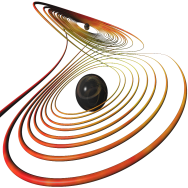
\includegraphics[height=16mm]{cgv-logo} \quad

\includegraphics[height=16mm]{tug-logo}
\end{center}
\end{titlepage}
\chapter{Abstract}

Häufig ist es notwendig, Algorithmen auf eine große Anzahl von \InputDateien{} anzuwenden.
Dabei ist es bei einer verteilten Ausführung nicht notwendig den Algorithmus zu parallelisieren.
Es ist ausreichend, den gegebenen Algorithmus auf mehreren Geräten mit unterschiedlichen Inputs zu starten.
Existierende Tools wie \MapReduce{} oder \ApacheSpark{} sind dafür ausgelegt Algorithmen zu parallelisieren, und dadurch komplexer als notwendig.
Diese Arbeit beschäftigt sich mit dem Design, der Implementierung und Evaluierung einer leichtgewichtigen JavaScript Middleware.
Die Eigenschaft “leichtgewichtig” bezieht sich auf den Sourcecode- und API-Umfang.
Tasks mit langen Laufzeiten erfordern aus Sicht der Usability die Möglichkeit abgebrochen zu werden, eine \ProgressAnzeige{} und Informationen über den Endzustand des ausgeführten Algorithmus.

Diese Arbeit analysiert zunächst bestehende und geeignete Konzepte und Technologien für eine solche Middleware und stellt danach eine Implementierung einer Middleware mit \JavaScript{}, \node{}, \Websockets{} und asynchronem API vor.
Da durchgehend ein asynchrones API verwendet wird, benötigen die auf der Middleware aufgebauten Anwendungen keine Synchronisierungsmechanismen wie zum Beispiel Semaphoren.
Die Skalierbarkeit dieses Prototypen wird in Kapitel \ref{K7} anhand eines \rgAlgorithmus{} und einer verteilten \PrimzahlenSuche{} analysiert und zeigt lineare Skalierbarkeit bis zu 16 Worker.

\tableofcontents

\mainmatter

% ------------------------------------------------------------
% =========================================================================
% CHAPTER 1
% =========================================================================

\chapter{Einleitung}

%==============================================================================

Die verteilte Ausführung von Algorithmen ist ein häufiger Lösungsansatz zur Minimierung ihrer Laufzeit.
Systeme wie MapReduce und Apache Spark haben in den letzten Jahren erheblich an Verwendung zugenommen.
Diese Systeme reduzieren den Deployment-Aufwand auf die Installation eines Interpreters auf den ausführenen Geräten und bieten dem Anwender dadurch eine stark vereinfachte Handhabung.
Denoch sind es Systeme die zur Verwendung sehr viel Wissen über die Technologie voraussetzen.

Muss ein Algorithmus auf viele Input-Dateien angewendet werden, ist es nicht notwendig den Algorithmus selbst zu parallelisieren.
Eine Ausführung auf mehreren Rechnern mit unterschiedlichen Input-Dateien ist ausreichend.
Für diesen Fall könnte ein System, das weniger Einarbeitungszeit als Apache Spark benötigt, gefunden werden.
Shell Scripts können diese Aufgabe übernehmen, allerdings nicht in heterogenen Netzwerken.
Remote Procedure Calls bieten ein einfaches API, sind aber nicht für Tasks mit langen Ausführungszeiten optimiert und von komplexen Deployment Schritten begleitet.
Bei Tasks mit langen Ausführungszeiten ist eine Progress-Anzeige und die Möglichkeit die Ausführung zu stoppen im praktischen Gebrauch notwendig, da es ansonsten zur Verschwendung von Rechner-Ressourcen und Wartezeiten kommt.
Auch aus Usability Gründen sind diese Features wünschenswert.

Ziel dieser Arbeit ist es, eine für oben genannte Aufgaben optimierte leichtgewichtige Middleware zu schaffen, die eine möglichst große Bandbreite an Geräten und Betriebssystemen abdeckt und ein einfaches Scripting API bietet.
Kapitel 2 zeigt die Ergebnisse einer Analyse verwandter Technologien und Themenbereiche.
Die für den Prototyp ausgewählten Technologien und Konzepte werden in Kapitel 3 aufgelistet und begründet.

Kapitel 4 und 5 dokumentieren das Design des Protokolls und Prototypen.
Dabei werden grundlegende Probleme und Lösungen der verteilten Programmierung, welche für diese Implementierung relevant sind, näher betrachtet.
Mit der Absicht auch andere Algorithmen mit diesem Tool verteilt auszuführen wurde ein Scripting API eingeführt, sodass der Prototyp in zwei Komponenten unterteilt werden kann:
in eine Middleware und dem Script das den gegebenen Algorithmus ausführt.
Im Zuge der Evaluierung wurden auch weitere Scripts geschrieben, wie zum Beispiel eine verteilte 3D Model Suche sowie eine verteilte Primzahlen-Suche.
Der entwickelte Prototyp verwendet JavaScript, Node.js, Websockets, und den Active Object Pattern um auf Basis einer Message Oriented Middleware remote Prozesse zu dirigieren.
Progress-Informationen werden über Betriebssystem-Pipes and die Middleware übergeben und von dieser an das auftraggebende Gerät weiter gereicht.
Die Input-Dateien und der Algorithmus müssen auf allen Rechnern zur Verfügung stehen.
Derzeit wird dafür ein verteiltes Dateisystem verwendet.

Eine Diskussion der Vor- und Nachteile des Designs erfolgt in Kapitel 6.
Da eine Bewertung der Simplizität des Scripting APIs formal nicht möglich ist, liegt der Schwerpunkt der Diskussion auf Skalierbarkeit.
Das Konzept ist auf einer niedrigeren Abstraktionsebene angesiedelt und lässt die Implementierung des Schedulers offen.
Desshalb werden in diesem Kapitel auch Eigenschaften des Systems und daraus resultierende Anforderungen an erweiterte Scheduler-Implementierungen gezeigt.
Anhand des 3D Processing Algorithmus wird in Kapitel 7 gezeigt, dass nur ein minimaler Overhead benötigt wird, sofern die Anzahl der mit einem Server verbundenen Worker klein bleibt.

% =========================================================================
% CHAPTER 2
% =========================================================================

\chapter{Ähnliche Arbeiten und Technologien}
\label{K2}
\section{Konzepte}

\subsection{Message-Oriented Middleware vs RPC}
Middleware Systeme können nach mehreren Gesichtspunkten klassifiziert werden.
Im Folgenden wird die Klassifizierung nach \cite{bishop2003survey} verwendet und auf die Klassen \sys{Procedure Oriented}, \sys{Object Oriented}, und \sys{Message-Oriented Middleware} eingegangen, da sie unter Berücksichtigung der Requirements mögliche Lösungsansätze sind.

\sys{Procedure Oriented} und \sys{Object Oriented} Systeme sind häufig als Request-Response  Protokolle implementiert, wie zum Beispiel Java RPC oder CORBA.
Einen Remote Call abzubrechen ist in diesem Kontext nur möglich, indem man die Ausführung an die TCP Connection bindet, das hieße die Ausführung abbzubrechen, falls die TCP Connection geschlossen wird.
Eine weitere Message für den Abbruch zu spezifizieren würde es ermöglichen, TCP Connections aufrecht zu erhalten wenn ein RPC abgebrochen wird.
Dies widerspricht aber dem Request-Response Konzept.
RPC Implementierungen wie \cite{qooxdoo} setzen dieses Konzept um.
Bei der Evaluierung von RPC Technologien konnte keine gefunden werden, die den Fortschritt der Ausführung am Client zur Verfügung stellt.
Um dies mit RPC zu realisieren, muss es im Application Layer implementiert werden.

\sys{Message-Oriented Middleware} Systeme bieten mehr Freiheit in der Hinsicht, dass Message-Sequenzen beliebig modelliert werden können.
Ein Remote Call mit Progress und Cancel Funktionalität kann relativ simpel mit vier Messages  modelliert werden:
Request, Progress, Cancel und Response.
Bei dieser Vorgehensweise muss jede der erwähnten Messages eine ID enthalten, welche auf den Aufruf verweist.

Beide Middleware Konzepte benötigen für die Progress und Cancel Funkionalität Implementierungen im Application Layer - eine Aufgabe, die dem Anwender abgenommen werden könnte.




\subsection{Asynchrone API}
Message-Oriented Middleware Systeme verwenden meist asynchrone APIs, während Procedure Oriented und Object Oriented Systeme meist synchrone APIs verwenden.
Es ist aber auch möglich, asynchrone APIs für RPC zu verwenden wie Falkner \cite{falkner1999implementing} gezeigt hat.

\label{future}
Asynchrone APIs, die mit Callbacks arbeiten, führen zu schwer lesbaren Code (pyramid of doom).
Um dies zu vermeiden können Futures und/oder Promises verwendet werden \cite{baker1977incremental}.
Promises sind Objekte, die das Ergebnis eines Funktionsaufrufs repräsentieren.
Bei den meisten Programmiersprachen kann dies neben dem Returnwert auch eine Exception sein.
Verwendet man Promises, wird das Ergebnis nicht durch Schlüsselwörter wie return oder throw definiert, sondern an das Promise Objekt übergeben.
So ist es möglich, auch innerhalb von Callbacks oder nach dem Verlassen der Funktion ein Ergebnis zu definieren.

Futures ergänzen dieses Konzept an der aufrufenden Stelle.
Asynchrone Funktionen geben beim Aufruf ein Future Objekt zurück.
Dieses kann verwendet werden um auf die Terminierung zu warten, beziehungsweise einen Eventhandler zu registrieren.
Wenn die asynchrone Funktion das Ergebnis an die Promise übergibt, gibt es diese an die Future weiter, welche in den Zustand Terminated übergeht.
Ist die Future in diesem Zustand, kann der Returnwert von ihr abgelesen werden \cite{baker1977incremental}.




\subsection{Active Object Pattern aka Actor Pattern}
Bei der Konzeptionierung von Serversystemen muss ein Threading Model gewählt werden.
Der Einsatz von multithreaded Modellen für ein Scripting API ist zu vermeiden, da es hohe Anforderungen an den Anwender im Bereich der Synchronisierung stellt.

Eine Möglichkeit Semaphoren zu vermeiden ist der Active Object Pattern \cite{schmidt2013pattern}.
Dieser verbindet eine Queue, in der Actions liegen, mit einem Thread welcher die Actions abarbeitet.
Es muss lediglich das Einfügen und Entfernen aus der Queue als atomare Operation ausgeführt werden.




\section{Technologien}

\subsection{Cluster- Grid- und Cloudcomputing}
Cluster, Grid und Cloud Computing haben eine Gemeinsamkeit:
Sie dienen der Nutzung von verteilten Ressourcen.
Ihre Unterschiede und die Abgrenzung zueinander sind nicht einheitlich definiert.
Im Folgenden wird die Klassifizierung nach \cite{sadashiv2011cluster} verwendet und ein kurzer Überblick in Bezug auf örtliche Ausdehnung, Ressourcen Allocation, Taskgröße, Heterogenität, Skalierbarkeit und Task Deployment gegeben.

Cluster Computing Systeme sind homogene, für lokale Netzwerke mit hohem Durchsatz optimierte Systeme.
Die Ressourcenverteilung wird von zentraler Stelle aus organisiert und limitiert damit die Skalierbarkeit.
Die Taskgröße ist nicht limitiert, dadurch eignen sie sich für verteilte Batch Verarbeitung.
Häufig wird MPI, eine Message Passing Middleware, verwendet.
Das Deployment der damit implementierten Programme ist nicht standardisiert und verlangt vom User detailliertes Wissen über den Cluster.

Grid Computing Systeme sind heterogene, für Netzwerke mit globaler Ausdehnung und geringem Durchsatz optimierte Systeme \cite{foster2003grid, foster2006grid}.
Typischerweise werden dabei mehrere lokale Netzwerke zu einem Grid verbunden, wodurch eine hierarchische Struktur entsteht.
Die Ressourcen Verteilung folgt ebenfalls dieser hierarchische Struktur, wodurch eine hohe Skalierbarkeit gegeben ist.
Die Taskgrößen sind nicht limitiert, dadurch eignen sie sich für verteilte Batch Verarbeitung.
Es existieren Erweiterungen wie MPICH-G2, die automatisches Job Deployment unterstützen.

Cloud Computing Systeme sind heterogene Systeme mit globaler Ausdehnung.
Sie sind für kleine Taskgröße designed und skalieren in Bezug auf die Anzahl dieser Tasks, aber nicht in Bezug auf die Große eines Tasks.
Diese Eigenschaft wird durch die Platform as a Service Eigenschaft erreicht, die das Task Deployment soweit vereinfacht, dass es on demand und automatisch geschehen kann.





\subsection{Apache spark}
Apache Spark ist ein Cluster Computing System, das auf einer MOM aufbaut.
Ein zu verteilender Algorithmus kann innerhalb eines Scripts implementiert werden.
Apache Spark API basiert auf Resilient Distributed Datasets (RDD).
RDDs bieten Methoden wie map, reduce, groupBy, filter und viele mehr.

Bei dem Aufruf dieser Funktionen unterteilt Apache Spark das RDD in Partitionen, wobei jeweils eine Partition von einem Worker verarbeitet wird.
Die hier als Beispiele genannten Methoden sind Funktionen höherer Ordnung, machen also klar, das auch ausführbarer Code an die Worker übergeben werden muss, damit dieser seine Partition abarbeiten kann.
Dies kann als versteckter Deployment Schritt gesehen werden und ist auch mit ein Grund für die einfache Handhabung von Apache Spark.

Darüber hinaus wird der User von technischen Details wie Fehlerkorrekturen und dem Versenden von Netzwerk Messages entbunden.
Apache  Spark unterstützt mehrere Persistenz Technologien, darunter HDFS, Hadoop und Cassandra \cite{zaharia2012resilient}.

% =========================================================================
% CHAPTER 3
% =========================================================================

\chapter{Anforderungen und verwendete Technologien}
\label{K3}
In diesem Kapitel werden zunächst die Anforderungen an die Middleware zusammengefasst. Danach die verwendeten Technologien und Konzepte aufgelistet und begründet, warum die Entscheidung auf sie gefallen ist.



\section{Anforderungen}

\BCL
  \item Es soll eine Middleware geschaffen werden, die auf einem möglichst großen Spektrum von Betriebssystemen und Geräten lauffähig ist.

  \item Der Deployment Aufwand soll minimiert werden.
  Ist die Middleware einmal auf den Geräten installiert, soll sie in der Lage sein Benutzer definierte Skripts verteilt auszuführen.

  \item Wie bei Apache Spark sollte der User nur ein Script schreiben müssen, welches das Ausführungsverhalten des gesamten Systems definiert, also auch den auf anderen Geräten ausgeführten Code enthält.
  Diese Scripts werden im folgenden \jobScript{} genannt.

  \item JobsScripts sollen es ermöglichen bei Funktionsaufrufen ein Gerät zu spezifizieren, auf dem die Funktion ausgeführt werden soll.

  \item Argumente und Returnwert oder Exceptions sollen von der Middleware transportiert werden.

  \item Auch das Starten von Remote Prozessen sollte auf dieses Art möglich sein.
  Solche Remote Calls werden im folgenden RemoteJobs genannt.
  Es wird angenommen, dass \remoteJobs{} mit einer sehr langen Ausführungszeit zum Einsatz kommen, deshalb müssen diese abbrechbar sein.
  Außerdem muss es möglich sein, den Progress von RemoteJobs an der auftraggebenden Stelle abzulesen.
\ECL

Es soll eine Middleware geschaffen werden, die auf einem möglichst großen Spektrum von Betriebssystemen und Geräten lauffähig ist.
Der Deployment Aufwand soll minimiert werden.
Ist die Middleware einmal auf den Geräten installiert, soll sie in der Lage sein Benutzer definierte Skripts verteilt auszuführen.
Wie bei Apache Spark sollte der User nur ein Script schreiben müssen, welches das Ausführungsverhalten des gesamten Systems definiert, also auch den auf anderen Geräten ausgeführten Code enthält.
Diese Scripts werden im folgenden \jobScript{} genannt.
JobsScripts sollen es ermöglichen bei Funktionsaufrufen ein Gerät zu spezifizieren, auf dem die Funktion ausgeführt werden soll.
Argumente und Returnwert oder Exceptions sollen von der Middleware transportiert werden.
Auch das Starten von Remote Prozessen sollte auf dieses Art möglich sein.
Solche Remote Calls werden im folgenden RemoteJobs genannt.
Es wird angenommen, dass \remoteJobs{} mit einer sehr langen Ausführungszeit zum Einsatz kommen, deshalb müssen diese abbrechbar sein.
Außerdem muss es möglich sein, den Progress von RemoteJobs an der auftraggebenden Stelle abzulesen.

Da bei RemoteJobs das Gerät explizit angegeben werden muss, muss innerhalb der Scripting Sandbox zumindest Zugriff auf die verbundenen, oder alle im Netzwerk zur Verfügung stehenden Geräte gegeben sein.
Somit kann der Anwender eigene Scheduling Strategien implementieren.
Pro Rechner muss CPU Auslastung, verfügbarer Speicher und verfügbare Interpreter abgelesen werden können.
Im Folgenden wird diese Datenstruktur \netInfo{} genannt.

Die Übertragung von sehr großen Datenmengen als Argument oder Returnwert ist nicht vorgesehen.
JobScripts sollten frei von Synchronisierungsmechanismen wie Semaphoren sein.




\section{Verwendete Technologien}

\subsection{ECMA Script aka JavaScript}
Ein JobScript enthält den Code aller beteiligten Geräte.
Funktion hohrere Ordnung enthalten Funktionen in der Argumentliste.
Bei Remote Aufrufen müssen die Argumente an die Gegenstelle gesendet werden, bei Porgrammiersprachen wie C++ ist es schwierig eine Serialisierbare Repräsentation einer Funktion zu erhalten.
Die Implementierung eines eigenen Compilers oder Präprozessors soll umgangen werden.
Programmiersprachen mit Reflection würden dies ermöglichen, allerdings mit erheblichem Aufwand.
\JavaScript{} macht es sehr einfach Stringrepräsentationen einer Funktion zu erhalten.

Javascript Interpreter sind auf nahezu allen Betriebssystemen vorhanden.
Auch mobile Endgeräte sind meist mit Browsern ausgestattet, die Javascript unterstützen.
Dadurch ist JavaScript eine der am häufigsten zur Verfügung stehenden Laufzeitumgebungen.
JavaScript unterstützt kein Multithreading - auf Servern ist es üblich Prozesse anstatt Threads zu verwenden.




\subsection{Websockets}
Für die Synchronisierung der \netInfo{} Datenstruktur muss bei Änderungen der Geräteeigenschaften eine Message an den Server und von diesem weiter an die Clients gesendet werden.
Vor allem das Weiterleiten an die Clients kann mit Websockets effizienter, das heißt ohne Polling, realisiert werden.
RemoteJobs müssen dem auftraggebenden Gerät Progress Updates zukommen lassen.
Auch hier kann Polling durch die Verwendung von Websockets vermieden werden.




\subsection{\node{} und \ActiveObjectPattern{}}
\JavaScript{} in Browsern und \node{} verwenden ein Threading Model, das einem \ActiveObjectPattern{} entspricht, wobei ein ganzer \node{} Prozess sowie ein Web Worker als \ActiveObjectPattern{} gesehen werden kann.
Darauf aufbauend kann eine MOM sehr einfach implementiert werden.
Um die Terminierung, das Abbrechen und Timeouts von RemoteJobs zu realisieren, muss eine \StateMachine{} auf Client- sowie Serverseite implementiert werden (siehe Kapitel \ref{K4}).
Die Transitions dieser State Machine werden durch Netzwerk Messages, User Inputs und Timer Events ausgelöst.

Da Webbrowser und \node{} kein Multithreading mit Shared Memory unterstützen, ist ein Asynchronous API unumgänglich.
Ein synchrones API würde entweder eine hohe Anzahl von Prozessen oder Web Worker benötigen, beziehungsweise starke Latenz Einbußen mit sich bringen.

%\subsection{MOM}

% =========================================================================
% CHAPTER 4
% =========================================================================

\chapter{Protokoll Design}
\label{K4}
Das hier beschriebene Protokoll ist für die Verwendung in einem hierarchischen Client-Server Overlay Network (HCSON) optimiert.
Da in einem solchen Netzwerk Jobs vom Client an den Server und von diesem an Worker gegeben werden, wird im Folgenden zwischen Auftraggeber und Auftragnehmer unterschieden, wobei der Server beide Rollen einnimmt.

Jeder teilnehmende Prozess besitzt eine global eindeutige ID, im Folgenden \NodeID{} genannt, und jeder Job egal ob remote oder nicht, erhält ebenfalls eine ID, im Folgenden \JobID{} genannt.
Alle Messages enthalten eine \JobID{} und beziehen sich jeweils auf genau einen Job.
Zudem enthält jeder Job die \JobID{} des ParentJobs, also jene des Jobs, von dem er erstellt wurde.

Alle Messages sind idempotent. Grundsätzlich entspricht eine Network Message einer State Machine Transition, nur die Return Message repräsentiert die returnOk, returnFail und returnCanceled Transitions. die Return Message enthält ein zusätzliches Flag, das zur Unterscheidung dient.




\section{Network Messages}
\label{messages}

\subsection{\CallMessage{}}
Call Messages werden vom Auftraggeber an den Auftragnehmer gesendet.
Sie enthalten JavaScript Code, der vom Empfänger ausgeführt wird und ersetzen so das Deployment.
Der Enthaltene Code hat seinen Ursprung im \ApplicationLayer{}, er wird beim Erstellen von Jobs definiert (siehe \ref{JobInterface}).

\subsection{\CancelMessage{}}
Cancel Messages werden vom Auftraggeber an den Auftragnehmer gesendet.
Cancel Messages führen nicht unbedingt zum Endzustand Canceled.
Falls der Auftraggeber bereits im Zustand Failed oder Ok ist, wird die Cancel Message ignoriert (siehe \ref{JobInterface}).

\subsection{\UpdateMessage{}}
Update Messages werden vom Auftragnehmer an den Auftraggeber gesendet.
Sie werden ausgelöst durch den Aufruf der \JobUpdate{} Funktion (siehe \ref{JobInterface}).
Update Messages enthalten den vom Auftragnehmer definierten Progress, optional eine für Menschen lesbare Statusinfo, sowie optionale Zwischenergebnise des Aufrufs.

\subsection{\ReturnMessage{}}
Diese Messages werden vom Auftragnehmer an den Auftraggeber gesendet, wenn der Job erfolgreich ausgeführt wurde, eine nicht behandelte Exception aufgetreten oder ein Timeout eingetreten ist.
Dies entspricht den Aufgaben von Futures (siehe \ref{future}, \ref{JobInterface}).
Return Messages können die State Machine Transitions returnOk, returnFail oder returnCanceled auslösen.
Ein Flag in der Message bestimmt die Transition.




\section{Job State Machine}
\label{jfsm}
Ein grundlegendes Problem von Distributed Computing ist es, am Client den Zustand von Remote Calls zu verfolgen.
Acknowledges können auf mehreren Layern zum Einsatz kommen, zum Beispiel nur am Tansport Layer.
In diesem Fall wird meist davon ausgegangen, dass eine erfolgreiche Übertragung auch zu einer erfolgreichen Ausführung führt.
\begin{wrapfigure}{L}{0.25\textwidth}
  \vspace{-20pt}
  \begin{center}
    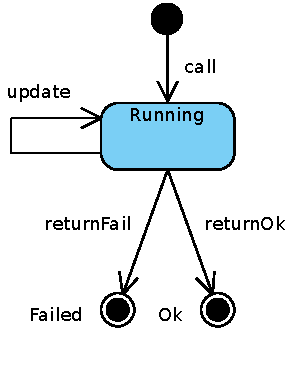
\includegraphics[width=0.25\textwidth]{fsm0}
  \end{center}
  \caption{State Machine eines nicht abbrechbaren RPC}
  \label{fsm0}
\end{wrapfigure}
Algorithmen, bei denen diese Annahme nicht getroffen werden kann, benötigen auch Acknowledges auf dem Application Layer.
Abbildung \ref{fsm0} zeigt eine simple State Machine für einen RPC der nicht abgebrochen werden kann.

An dieser Stelle sollte beachted werden, dass auch diese State Machine verteilt ist.
Sie stellt den Zustand des Remote Calls dar, dieser existiert real am Client und am Server.
Oder mit anderen Worten: Dieser Zustand wird im Stub und im Skeleton gehalten.
Entsprechende Netzwerk Messages synchronisieren den Zustand zwischen Client und Server.
Die \TransReturnOk{} emittiert eine positive \ReturnMessage{}, die \TransReturnFail{} emittiert eine negative \ReturnMessage{}.
Die \TransCall{} wird durch eine \CallMessage{} ausgelöst.

Auch für den Fall, dass kein Abbruch des RPC unterstützt wird und der Server nur am Ende der Ausführung eine Message mit dem Erfolgszustand an den Client sendet, ist es nicht immer möglich, diese State Machines zu synchronisieren. Siehe Zwei-Armeen-Problem \cite{tanenbaum4andrew}.
Denn der Client könnte durch ein Timeout Event, das genau dann eintritt, wenn die Return Message vom Server auf dem Weg zum Client ist, in den Failed Zustand übergehen, während der Server bereits im Ok Zustand ist.

Wird das System so erweitert, dass Remote Calls abgebrochen werden können (siehe Abbildung \ref{fsm1}), trifft man auf dasselbe Problem wenn vom Client eine Abbruch Meldung an den Server gesendet wird und der Server bereits eine Erfolgsmeldung gesendet hat, diese aber noch nicht am Client angekommen ist.
\begin{wrapfigure}{R}{0.45\textwidth}
  \vspace{-20pt}
  \begin{center}
    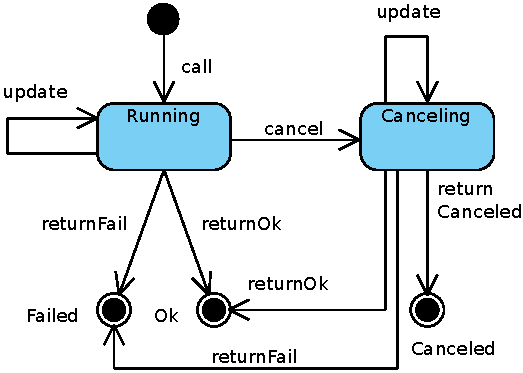
\includegraphics[width=0.45\textwidth]{fsm1}
  \end{center}
  \caption{Erweiterte State Machine eines abbrechbaren RPC}
  \label{fsm1}
\end{wrapfigure}
Eine Strategie um dieses Problem zu minimieren ist es, den Client nicht in den Canceled State übergehen zu lassen ohne vom Server eine Bestätigung erhalten zu haben.
Im Detail bedeutet das, dass der Client in den Canceling State übergeht, eine Nachricht an den Server sendet mit dem Auftrag die Ausführung abzubrechen und dann vom Server den Endzustand erhält.
Soweit scheint es, dass beide am Ende im selben Zustand sind, jedoch muss auch der Canceling State mit einem Timeout überwacht werden, was wiederum zum Zwei-Armeen-Problem führt.

Will man nicht nur am Ende der Ausführung vom Server über dessen Zustand informiert werden, sondern auch während der Ausführung, zum Beispiel über den Progress oder Warnings, so können ebenfalls Race Conditions beim Abbruch auftreten, wenn nicht diese Art der Terminierung verwendet wird.
Der Client könnte durch ein Timeout bereits im Failed State sein, während der Server noch Running States publiziert.

Dabei wird auch offensichtlich, dass Ressourcen verschwendet werden,  während am Client bereits davon ausgegangen wird, dass die Ausführug fehlgeschlagen ist, der Server aber noch daran arbeitet.
In diesem Fall können Ergebnisse nicht vom Client angenommen werden, weil am Client die Ausführung bereits als Fehlerhaft deklariert wurde.

Die Verschwendung dieser Ressourcen kann minimiert werden, in dem der Client im Fall eines Timeouts den Remote Call am Server durch eine Cancel Message beendet
- minimiert deshalb, weil immer noch Netzwerkfehler einen solchen Abbruch verhindern können.
Im Folgenden werden Remote Calls, welche diese State Machine implementieren, Jobs genannt.
Jobs können aber auch rein lokal für asynchrone Aufrufe verwendet werden.
Der das handling von verlorenen Messages ist in diesem Fall zwar nicht notwendig, dennoch können sie hilfreich sein beim auffinden von Implmentierungsfehlern und Race Conditions (siehe Kapitel \ref{K5}).





\section{JobTrees und Call Graphen}
In einem HCSNO ist es üblich Aufgaben zu delegieren. Der Client gibt Aufträge an den Server, der Server an die Worker.
Die einzelnen durchlaufenen Code Stücke können als Directed Acyclic Graph (DAG), der Ahnlichkeiten zu einem lokalen Call Graphen hat, dargestellt werden \cite{yu2005taxonomy}.
Dieser DAG beschreibt den durchlaufenen Workflow über alle Rechner.
In P2P Netzwerken können diese Graphen noch größere Tiefen erreichen.
Jedem Knoten im DAG ist eine Workflow Logic zugeordnet. Typische Workflows sind:
\BCL
  \item Worker werden parallel gestartet und müssen alle erfolgreich terminieren
  \item Worker werden parallel gestartet, einer muss erfolgreich sein (Redundanz)
  \item Worker werden konsekutiv gestartet, alle müssen erfolgreich sein
  \item Pooling. N Worker arbeiten parallel, jedoch gibt es mehr Aufträge als Worker. Schließt ein Worker einen Job ab, beginnt er mit einem der übrigen Jobs, bis alle abgearbeitet wurden
\ECL
Die Vollständigkeit dieser Liste ist nicht gegeben.
Der Anwender muss also die Möglichkeit haben, diese Liste zu erweitern.
Die Javascript Bibliothek async \cite{async} verwendet ein ähnliches Konzept für asynchrone Funktionsaufrufe, und zeigt eine beeindruckende Liste an möglichen Workflows.

Der Workflow DAG dieser Implementierung wird im folgenden JobTree genannt.
Jeder Knoten im JobTree ist eine Job State Machine.
Delegiert ein Job A eine Aufgabe an einen anderen Job B, wird A im folgenden \ParentJob{}, und B \SubJob{} genannt.

Hat ein Knoten in einem Call Graphen mehrere Kinder, bedeutet dies immer sie wurden Konsekutiv ausgeführt.
Im Kontext dieser Arbeit muss es möglich sein Unteraufgaben parallel auszuführen, genauer betrachtet muss es sogar möglich sein den Startzeitpunkt für jede Unteraufgabe frei festzulegen (siehe Pool Workflow).
Die Implementierung des Prototypen verwendet einen Strategy Pattern um den Anwender der Middleware die Möglichkeit zu geben eigene Startsequenzen zu definieren.

Der Zustand des ParentJobs ist von den Zuständen der SubJobs, und der ParentJob Terminate Strategy abhängig.
Die angestrebte Vereinfachung des Middleware APIs  beruht im Wesentlichen darauf, dass die Implementierung des Workflows nicht im Application Layer statt findet, sondern das eine SubJob Start Strategy und eine ParentJob Terminate Strategy aus einer Menge von vordefinierten  Strategien ausgewählt wird.






\begin{wrapfigure}{r}{0.3\textwidth}
  \vspace{-55pt}
  \begin{center}
    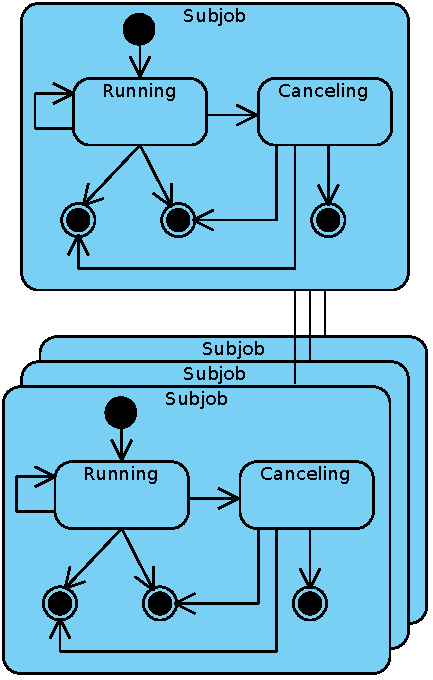
\includegraphics[width=0.3\textwidth]{hfsm}
  \end{center}
  \label{hfsm}
  \caption{Immer wenn eine der untergeordneten State Machines terminiert, wird der Workflow Logic Terminate Strategie aufgerufen.
  Dieser entscheidet ob die Übergeordnete State Machine ihren State ändern muss.}
\end{wrapfigure}
\section{Hierarchische Job State Machine}
Soll ein Job, zum Beispiel am Server, nur die geeigneten Worker ermitteln und die ihm übergebene Aufgabe an diese delegieren, kann die Funktion \JobDelegate{} verwendet werden um dem Job SubJobs hinzuzufügen.
\JobDelegate{} erwartet eine ParentJob Terminate Strategy, eine SubJob Start Strategy, sowie eine Liste der Subjobs.
Anstatt der Liste der SubJobs kann auch eine Factoryfunktion verwendet werden.
\JobDelegate{} bindet Die State Machine des ParentJobs and die der SubJobs, es entsteht eine hierarchische FSM (siehe Abbildung \ref{hfsm}).

Der Aufruf von \JobDelegate{} führt die SubJob Start Strategy aus.
Diese kann nun entscheiden welche SubJobs gleich zu Beginn gestartet werden sollen.
Terminiert ein SubJob wird die ParentJob Terminate Strategy aufgerufen.
Diese muss zunächst entscheiden ob der Parent terminieren soll, wenn nicht kann sie bei bedarf weitere SubJobs starten (siehe Abbildung \ref{seq}).

Wird der ParentJob abgebrochen, wird die \CancelMessage{} an die SubJobs weiter gegeben. Auf Application Layer ist keine Implementierung notwendig.
Terminiert der ParentJob werden et­wa­ige noch laufende SubJobs ebenfalls abgebrochen.
Da bekannt ist wieviele SubJobs vorhanden sind, und welche davon bereits terminiert haben, kann der Progress des ParentJobs bestimmt werden.
Dieses Konzept sollte auch bei P2P Network Overlays anwendbar sein.

JavaScript Promises unterstützen ein ähnliches Konzept.
Promise.race wird für den Fall, dass eine erfolgreiche sub Promise ausreichend ist verwendet und Promise.all für den Fall, dass die erfolgreiche Ausführung aller sub Promises obligat ist.

\begin{wrapfigure}{R}{1\textwidth}
  \vspace{-20pt}
  \begin{center}
    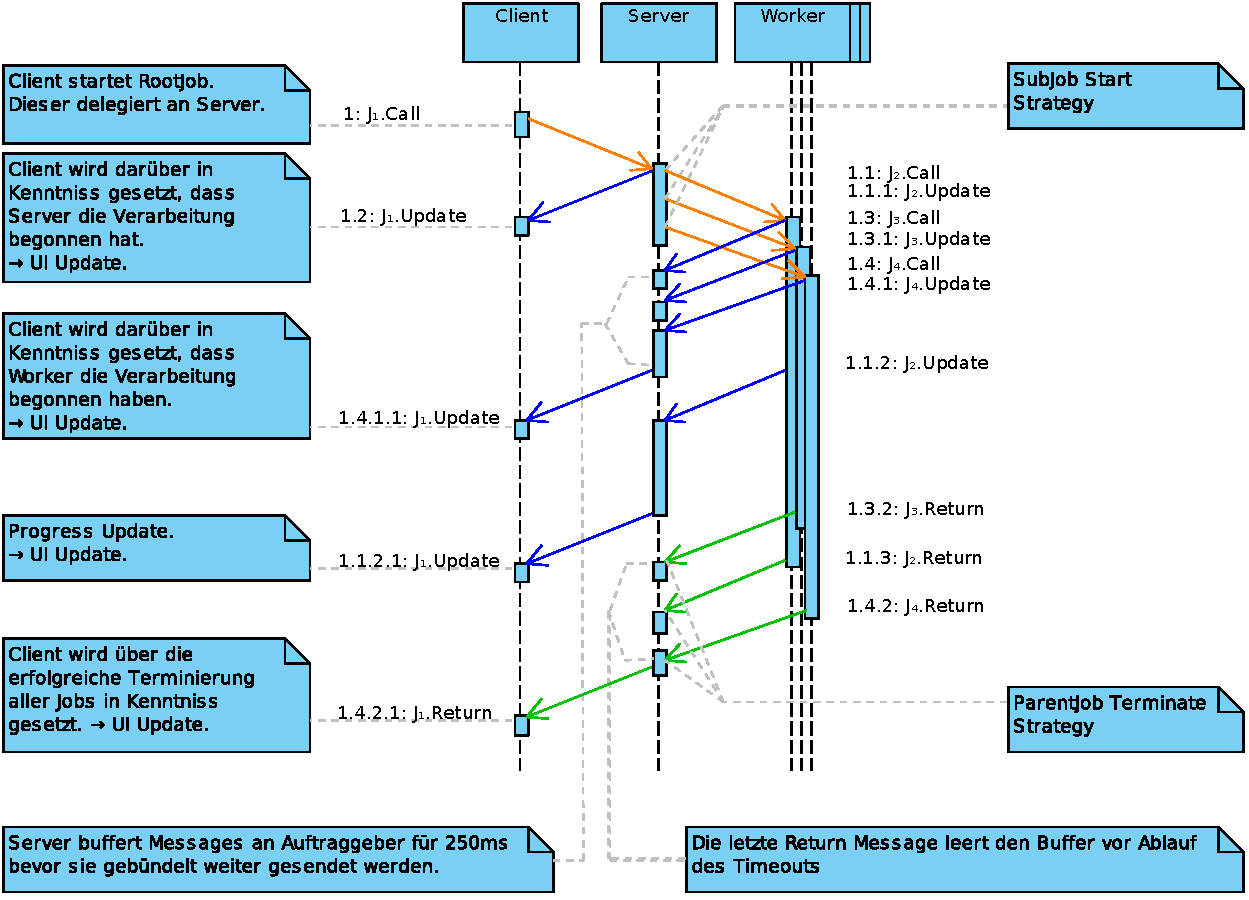
\includegraphics[width=1\textwidth]{seq}
  \end{center}
  \caption{UML Sequenz Diagramm eines Parallel Workflows. Einfachster Fall ohne Fail oder Cancel Messages.PartentJob terminiert wenn alle SubJobs terminiert haben. $J_1$ ist RootJob, und zugleich ParentJob von $J_2$, $J_3$ und $J_4$. Orange sind Call Messages, Blau Update Messages und Grün ReturnOk Messages.}
  \label{seq}
\end{wrapfigure}

% =========================================================================
% CHAPTER 5
% =========================================================================

\chapter{Software Design}
\label{K5}
\section{Deployment}
\begin{wrapfigure}{r}{0.275\textwidth}
  \vspace{-24pt}
  \begin{center}
    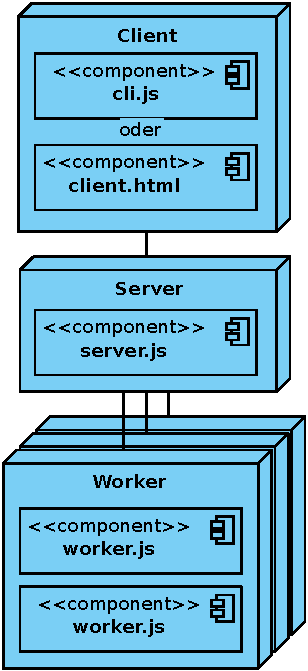
\includegraphics[width=0.275\textwidth]{deploy}
    \caption{UML Deployment Struktur mit Netzwerk Verbindungen. Client ist entweder CLI-Client oder
     Webclient.}
    \label{fig:deploy}
  \end{center}
  \vspace{-50pt}
\end{wrapfigure}

Die Implementierung besteht aus mehreren ausführbaren Komponenten: ein CLI-Client, Webclient, dem Server und den Workern (siehe Abbildung \ref{fig:deploy}).
Im Folgenden werden Instanzen dieser als Node bezeichnet.
Bis auf den Webclient sind sie alle als Node.js Script ausgeführt.

Die Unterschiede dieser Komponenten sind gering.
CLI-Client und Webclient unterscheiden sich von den anderen Komponenten nur durch das zusätzlich enthaltene UI.
Die Worker unterscheiden sich vom Server nur dadurch, dass sie ClientWebSockets anstatt ServerWebsockts verwenden.
Dieses Design wurde gewählt, um zukünfigte arbeiten mit P2P und HCSNO mit mehreren Worker Ebenen zu erleichtern.

Ansonsten hat jede dieser ausführbaren Komponenten intern den gleichen Aufbau, welcher in den folgenden Abschnitten beschrieben wird.




\section{NetInfo}
Als ein globales Objekt ausgeführt, steht diese Komponente in allen Modulen zur Verfügung, auch in JobScripts.
Verwendung findet sie vor allem in JobScripts, um geeignete Worker auszuwählen.
Das NetInfo Objekt besteht aus einer Liste der im System vorhandenen Nodes.
Jede Node darin bietet folgende Eigenschaften:
\BCL
  \setlength\itemsep{0.0em}
  \item Funktionen zum Empfangen und Senden von Daten
  \item Momentane CPU- und Speicherauslastung
  \item Informationen über das Betriebssystem
  \item Liste der auf dem Gerät installierten Interpreter
\ECL
\noindent Um CPU- und Speicherauslastung aktuell zu halten, senden alle Teilnehmer zyklisch Updates an den Server.
Dieser leitet sie an die Clients weiter.
Derzeit ist noch keine Publish-Subsribe Implementierung vorhanden, sollte aber verwendet werden, um die Netzwerkauslastung zu minimieren.
Die Struktur des Network Overlays ist durch Konfiguration definiert, Clients und Worker verbinden sich mit dem Server, wodurch ein HCSNO entsteht.




\section{App}
Eingehende Nachrichten werden an das App Modul weiter gegeben.
Zunächst ist es dessen Aufgabe, den zur Nachricht gehörenden Job zu finden, beziehungsweise einen neuen zu erstellen falls es eine Call Nachricht ist.
Wie in Kapitel \ref{K4} beschrieben, enthalten die Nachrichten JavaScript Code, welcher vom App Modul in einer Sandbox ausgeführt wird.
Innerhalb dieser Sandbox stehen der Job, das NetInfo Objekt, die Job- und Tooljob-Implementierungen zur Verfügung.




\section{Job Interface}
\label{JobInterface}
Die abstrakte Job Klasse implementiert die in Kapitel \ref{jfsm} beschriebenen State Machine.
State Transitions werden mit den Funktionen call, cancel, update und return ausgelöst.
Die Implementierung der Job Klasse ist verantwortlich für das Abfangen von nicht erlaubten Transitions und für Timeouts.
Sie führt die abstrakten Funktionen onCall, onCancel, onUpdate, onReturn zur jeweiligen Transition aus.
Die Implementierungen  dieser Funktionen werden im Konstruktor übergeben.

onCall muss definiert werden, onCancel, onUpdate und onReturn sind optional.
Im Vergleich zu JavaScript Promises entspricht onCall der dem Konstruktor übergebenen Funktion.
onReturn übernimmt die Aufgaben der reject und resolve Funktionen.
onCancel und onUpdate existieren bei JavaScript Promises nicht, da diese nicht abbrechbar sind und zu onUpdate gibt es kein Äquivalent, da Promises keine Zwischenergebnisse liefern können.

Ein laufender Job muss früher oder Später retournieren.
Das kann entweder duch einen Aufruf von \JobReturn{} geschehen, nachdem er seine Aufgabe erfüllt hat,
oder der Job ist an SubJobs gebunden, und es wird von der Workflow Logic aufgerufen wenn die SubJobs ihre Aufgaben erfüllt haben.
Abbildung ŗef{code} zeigt zwei Jobs die durch die Workflow Logic geschlossen werden (j und js),
und weitere (jw, die Leafs im JobTree) die durch einen \JobReturn{} Aufruf terminiert werden.





\section{RemoteJob, AjaxJob und SpawnProcessJob}
Die in \ref{JobInterface} beschriebene Klasse ist abstrakt und dafür vorgesehen vom Anwender spezialisiert zu werden.
Dieser Abschnitt beschreibt drei in der Middleware enthaltenen Spezialisierungen (Ableitungen).

RemoteJobs führen die onCall Funktion auf einem Remote Gerät aus.
Es muss eine Node aus dem NetInfo Objekt ausgewählt und an den Konstruktor des RemoteJobs übergeben werden.
call, cancel, update und return führen ihre zugehörigen ‘on*’ Funktionen nicht direkt aus, sondern übertragen eine String-Representation der Funktion an das Remote Gerät, wo sie vom App Modul interpretiert werden.
Weitere Tooljobs wie AjaxJob und SpawnProcessJob adaptieren die bestehende Technologien XMLHttpRequest und das Node.js Process Interface, damit sie in JobTrees eingesetzt werden können.




\section{Jobscripts}

\begin{wrapfigure}{r}[10mm]{0.75\textwidth}
  \vspace{-10mm}

  \begin{center}
    \fvset{frame=single,framesep=0mm,fontsize=\small,fontfamily=courier,numbers=left,xleftmargin=5mm,xrightmargin=10mm,framerule=.1mm,numbersep=1mm,commandchars=\\\{\},codes={\catcode`$=3\catcode`^=7\catcode`_=8}}
    \hspace{-5cm}
    \begin{Verbatim}

\textcolor{BlueViolet}{  var onCallScript = \textbf{j=>} j.delegate(\{}
\textcolor{BlueViolet}{      onlyOne:true,}
\textcolor{BlueViolet}{      job: ()=> \textbf{new RemoteJob}(\{}
\textcolor{BlueViolet}{          desc: 'init workers on server',}
\textcolor{BlueViolet}{          node: network.connections[0],}
\textcolor{BlueViolet}{          args: j.params,}
\textcolor{BlueViolet}{          onCallRemote:}\textcolor{OliveGreen}{ \textbf{js=>} js.delegate(\{}
\textcolor{OliveGreen}{              workerPool: getNodesByCapability('POSIX64'),}
\textcolor{OliveGreen}{              jobCount: 20,}
\textcolor{OliveGreen}{              job: (idx, poolnode)=> \textbf{new RemoteJob}(\{}
\textcolor{OliveGreen}{                  desc: 'empty job on worker',}
\textcolor{OliveGreen}{                  node: poolnode,}
\textcolor{OliveGreen}{                  args: \{\},}
\textcolor{OliveGreen}{                  onCallRemote:}\textcolor{Mahogany}{ \textbf{jw=>} jw.ret('ok', 'empty')}
\textcolor{OliveGreen}{              \})}
\textcolor{OliveGreen}{          \})}
\textcolor{BlueViolet}{      \})}
\textcolor{BlueViolet}{  \})}

    \end{Verbatim}
  \end{center}
  \caption{Ein JobScript das 20 leere Jobs auf Workern ausführt. \textcolor{White}{- - -} \protect\linebreak Blau: Client, Grün: Server, Rot: Worker.}
  \label{code}
\end{wrapfigure}

Der RootJob wird immer vom UI erzeugt.
JobScripts enthalten eine Einstiegsfunktion, die beim Aufruf den RootJob im State Running als Parameter erhält.
Das UI ist dann bereits an den RootJob gebunden und zeigt zumindest seinen Zustand.

Die Skript Funktion enthält Code von Client, Server und Worker.
Abbildung \ref{code} zeigt ein Script, dass 20 ‘leere’ Jobs auf Worker Nodes ausführt.

\ref{code} Zeile 9 zeigt die Auswahl der Worker die den Pool bilden.
getNodesByCapability ist eine Toolfunktion die alle 64bit Posix kompatiblen Nodes aus der NetInfo Datenstruktur liefert. Bevor der WorkerJob retouniert wird für gewöhnlich dessen Aufgabe ausgeführt.

\begin{wrapfigure}{r}{1\textwidth}
  \begin{center}
    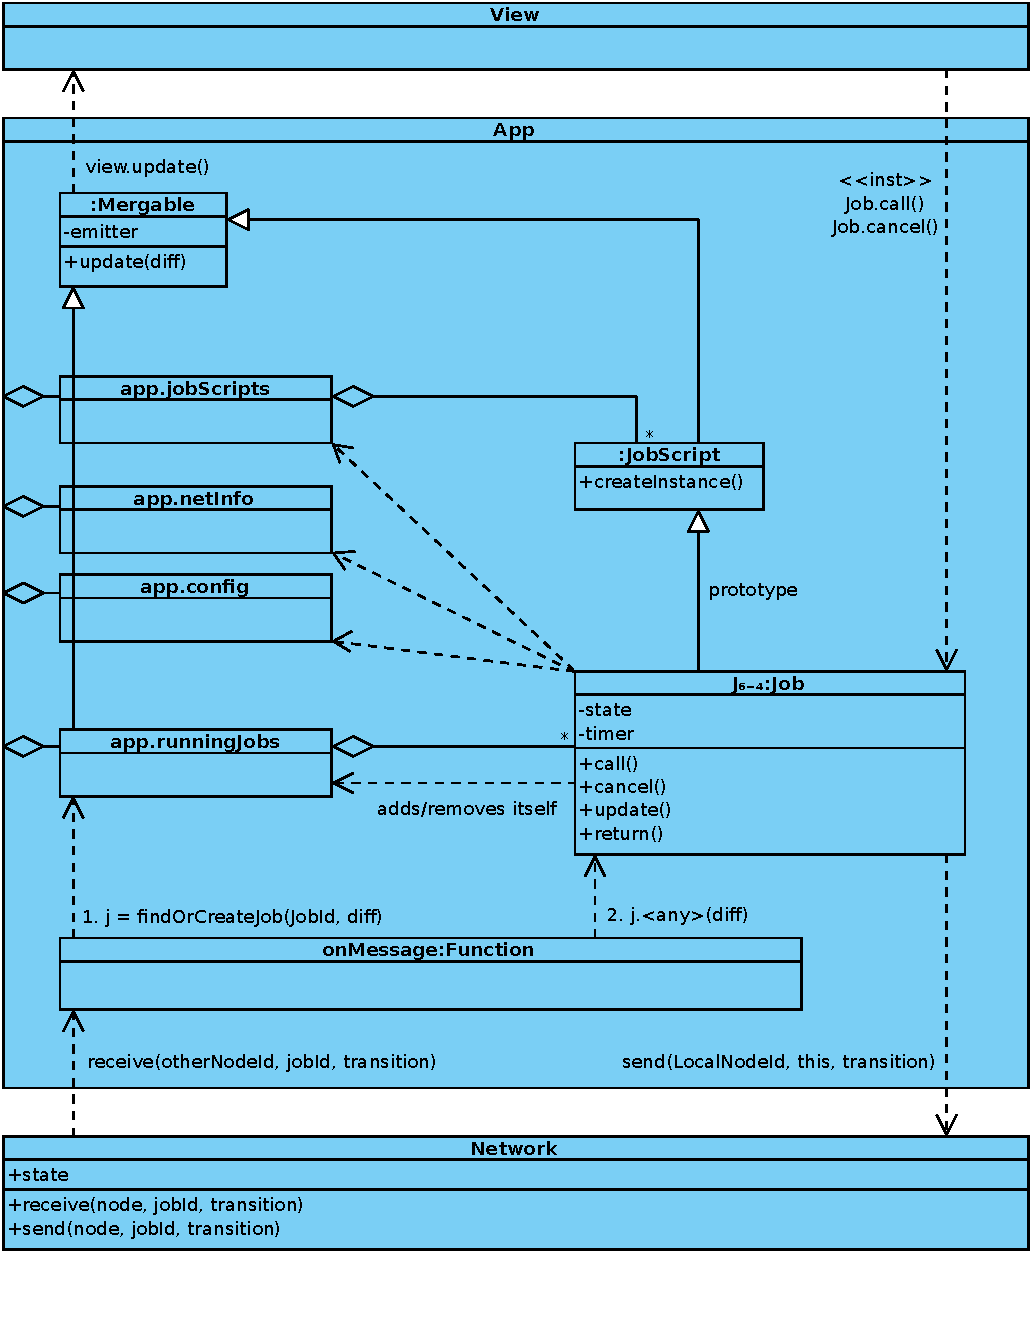
\includegraphics[width=0.9\textwidth]{vm}
  \end{center}
  \label{deploy}
  \label{viewModel}
  \caption{UML Object Diagramm des Client. Server and Worker enthalten keine View. }
\end{wrapfigure}

% =========================================================================
% CHAPTER 7
% =========================================================================

\chapter{Evaluierung}
\label{K7}

Dieses Kapitel evaluiert den \textit{pool} und \textit{parallel} Workflow mit mehreren \jobScript s.
Der Webclient wird verwendet um einzelne Test Jobs auszuführen, das CLI um Test Jobs 25 mal auszuführen.
Gemessen wurden neben der Gesamtlaufzeit (\RootJob{} Laufzeit) auch die Laufzeiten der WorkerJobs.
Joblaufzeiten werden immer auf dem Rechner auf dem der Job erstellt wurden gemessen, für \remoteJob s bedeutet das inklusive des Netzwerk Roundtrips.
Das System wird mit beiden Clients einem Stresstest unterzogen, indem WorkerJobs mit minimaler Laufzeit (sie terminieren sobald das onCall Event aufgerufen wird) eingesetzt werden (\ref{M3}, \ref{overload}).
Dieser Stresstest wird mit dem Pool Workflow durchgeführt, da er mehr Netzwerk Messages benötigt.

Ziel der CLI Messungen ist es zu zeigen, dass das \jobScript{} skaliert (\ref{M1}, \ref{M2}).
Jeder Test führt einen Job auf 1, 2 und 4 Worker Devices aus. Auf jedem Worker Device laufen 4 Worker Nodes.
Verteilte Systeme sind nicht zeitlich deterministisch, desshalb werden alle Messungen 25 mal wiederholt.
Die Skalierbarkeit wird mit einem Boxplot der Gesamtlaufzeit mit linearen Achsen, und einem mit logaritmischen Achsen veranschaulicht.
%histogramme der WrokerJobs zeigen unmgebungs eigenschaften, beschreiben vorgangn, lassen auf fehler schließen

Webclient Tests führen ihren Test Job nur ein mal aus.
Der Webclient ist in der lage Gantcharts aus \JobTree s zu generieren.
Diese werden genutzt um die Probleme aufzuzeigen die beim implementieren von \jobScript s entstehen können (\ref{schedulerNeeded}, \ref{overload}).

%ein Script, das einen Bereich der natürlichen Zahlen nach Primzahlen durchsucht (siehe Experiment \ref{M1}),
%und ein weiteres, das einen \rgAlgorithmus{} auf mehrere Input-Dateien anwendet (siehe Experiment \ref{M2}, \ref{M3}).

\begin{table}[H]
\centering

\begin{tabular}{|l|l|l|l|r|r|r|}
\hline
\multicolumn{7}{|l|}{}                                                                                                                                           \\
\multicolumn{7}{|c|}{Webclient Tests}                                                                                                                            \\
\multicolumn{7}{|l|}{}                                                                                                                                           \\ \hline
Abschnitt                             & Wiederh.            & Workflow                  & WorkerJobs          & Worker Nodes & Worker Devices & mean(T) {[}ms{]} \\ \hline
\multirow{3}{*}{\ref{M1} \thumbsup}   & \multirow{9}{*}{25} & \multirow{3}{*}{Parallel} & 4                   & 4        & 1          & 7 004                    \\ \cline{4-7}
                                      &                     &                           & 8                   & 8        & 2          & 3 706                    \\ \cline{4-7}
                                      &                     &                           & 16                  & 16       & 4          & 2 342                    \\ \cline{1-1} \cline{3-7}
\multirow{3}{*}{\ref{M2} \thumbsup}   &                     & \multirow{3}{*}{Pool}     & \multirow{3}{*}{65} & 4        & 1          & 672 136                  \\ \cline{5-7}
                                      &                     &                           &                     & 8        & 2          & 332 253                  \\ \cline{5-7}
                                      &                     &                           &                     & 16       & 4          & 154 961                  \\ \cline{1-1} \cline{3-7}
\multirow{3}{*}{\ref{M3}}             &                     & \multirow{3}{*}{Pool}     & \multirow{3}{*}{20} & 4        & 1          & 103                      \\ \cline{5-7}
                                      &                     &                           &                     & 8        & 2          & 120                      \\ \cline{5-7}
                                      &                     &                           &                     & 16       & 4          & 118                      \\ \hline
\multicolumn{7}{|l|}{}                                                                                                                                           \\
\multicolumn{7}{|c|}{CLI Tests}                                                                                                                                  \\
\multicolumn{7}{|l|}{}                                                                                                                                           \\ \hline
Abschnitt                             & Wiederh.            & Workflow                  & WorkerJobs          & Worker Nodes & Worker Devices & T {[}ms{]}       \\ \hline
\ref{schedulerNeeded}                 & \multirow{2}{*}{1}  & Pool                      & 12                  & 3        & 1          & 21 209                   \\ \cline{1-1} \cline{3-7}
\ref{overload}                        &                     & Pool                      & 20                  & 3        & 1          & 1 064                    \\ \hline
\end{tabular}

\caption{Test Übersicht. Grüner Daumen markiert lineare Skalierbarkeit.}
\label{testtable}
\end{table}


\noindent Als Hardware standen fünf Rechner mit gleicher Ausstattung, jeweils 4 Cores und 16GB RAM, zur Verfügung.
Pro Rechner wurden maximal vier Worker verwendet um Swapping zu vermeiden, denn die \jobScript s verwenden nur einen primitiven \scheduler{}.
Als Betriebssystem wurde Debian Linux verwendet.
Experiment \ref{M2} startet WorkerJobs die auf ein verteiltes Dateisystem (AFS) zugreifen. AFS cached die Lesevorgänge.

%Für die folgenden Experimente wird jeweils ein Histogram der WorkerJob Laufzeiten und ein Boxplot der Gesamtlaufzeit für ein, zwei und vier Rechner gezeigt.
%Weiters wird die Gesamtlaufzeit über der Rechneranzahl auch mit logarithmischen Achsen gezeigt, da in dieser Darstellungsform eine lineare Funktion die lineare Skalierbarkeit besser sichtbar macht.


















\clearpage
\section{CLI Tests}

\subsection{Primzahlen Suche - Parallel Workflow}
\label{M1}

\begin{wrapfigure}{r}{0.45\textwidth}
  \vspace{-30pt}
  \begin{center}
    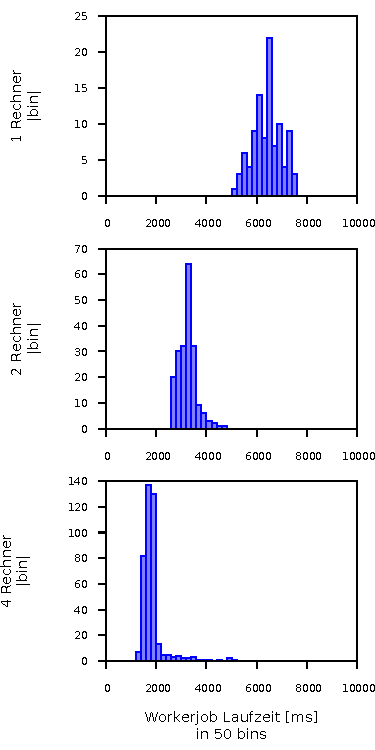
\includegraphics{hist-workerPrimeCpp}
    \caption{Experiment \ref{M1} WorkerJob Laufzeiten aller 25 Iterationen in 50bins.}
    \label{hist-workerPrimeCpp}
  \end{center}
\end{wrapfigure}

%#WorkerJobs
%was amcht ein Workerjob
%IO
%avg(T)
%#messages
%parameter

Dieses Experiment wurde ausgewählt, weil es einen sehr einfachen Fall zeigt, der auch gut skaliert.
Der Algorithmus duchsucht den Bereich $10^{7}$ bis $2 \cdot 10^{7}$ nach Primzahlen und übergibt die Anzahl der gefundenen Primzahlen zusammen mit dem Progress in Echtzeit an den Client.
Die WorkerJobs sind in C++ implementiert, und benötigen keinen Dateisystem IO.
Für Laufzeiten siehe Tabelle \ref{testtable}.

Der Serverteil des \jobScript s teilt den zu durchsuchenden Bereich proportional auf die zur Verfügung stehenden Worker auf.
Somit ist die Anzahl der WorkerJobs immer gleich der Anzahl der Worker.
Stehen mehr Worker zur Verfügung, wird der zu durchsuchende Bereich für jeden Worker kleiner.
Histogramm \ref{hist-workerPrimeCpp} zeigt, dass mittlere WorkerJob Laufzeit annähernd linear mit der Anzahl der verfügbaren Worker sinkt.
Die Gesamtlaufzeit zeigt die erwartete lineare Skalierbarkeit, ersichtlich in Abbildung \ref{runtime-box-workerPrimeCpp} und \ref{runtime-log-workerPrimeCpp}.

Das Messaging Verhalten zwischen Server und Worker benötigt nur einen Roundtrip je Worker Node.
Zu begin sendet der Server eine \CallMessage{} an jede Worker Node, diese senden im 250ms Intervall \UpdateMessage s an den Server, und am Ende möglichst gleichzeitig jeweils eine \ReturnMessage.

Der parallel Workflow skaliert nur dann linear, wenn alle WorkerJobs gleich große Laufzeiten aufweisen.
Bei der Primzahlensuche ist dies im Detail betrachet nicht der Fall, weil großere Zahlen eine größere Laufzeit veruhrsachen und die Zahlen im letzten Block größer sind.


\vspace*{\fill}

\begin{figure}[H]
  \centering
  \begin{minipage}[b]{0.45\textwidth}
    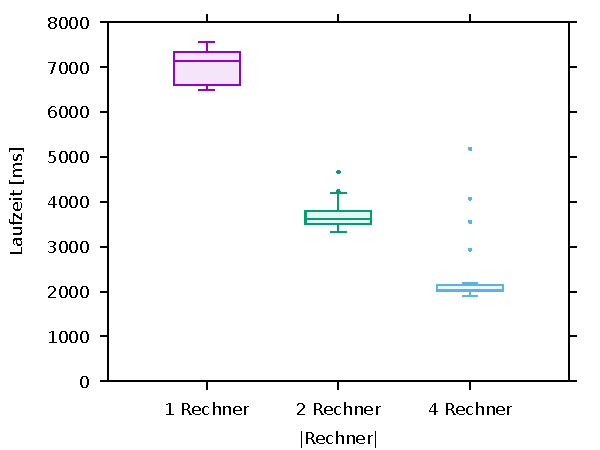
\includegraphics[width=\textwidth]{runtime-box-workerPrimeCpp}
    \caption{Experiment \ref{M1}. Boxplots für Gesamtlaufzeit mit 1, 2, und 4 Worker, und je 25 Iterationen}
    \label{runtime-box-workerPrimeCpp}
  \end{minipage}
  \hfill
  \begin{minipage}[b]{0.45\textwidth}
    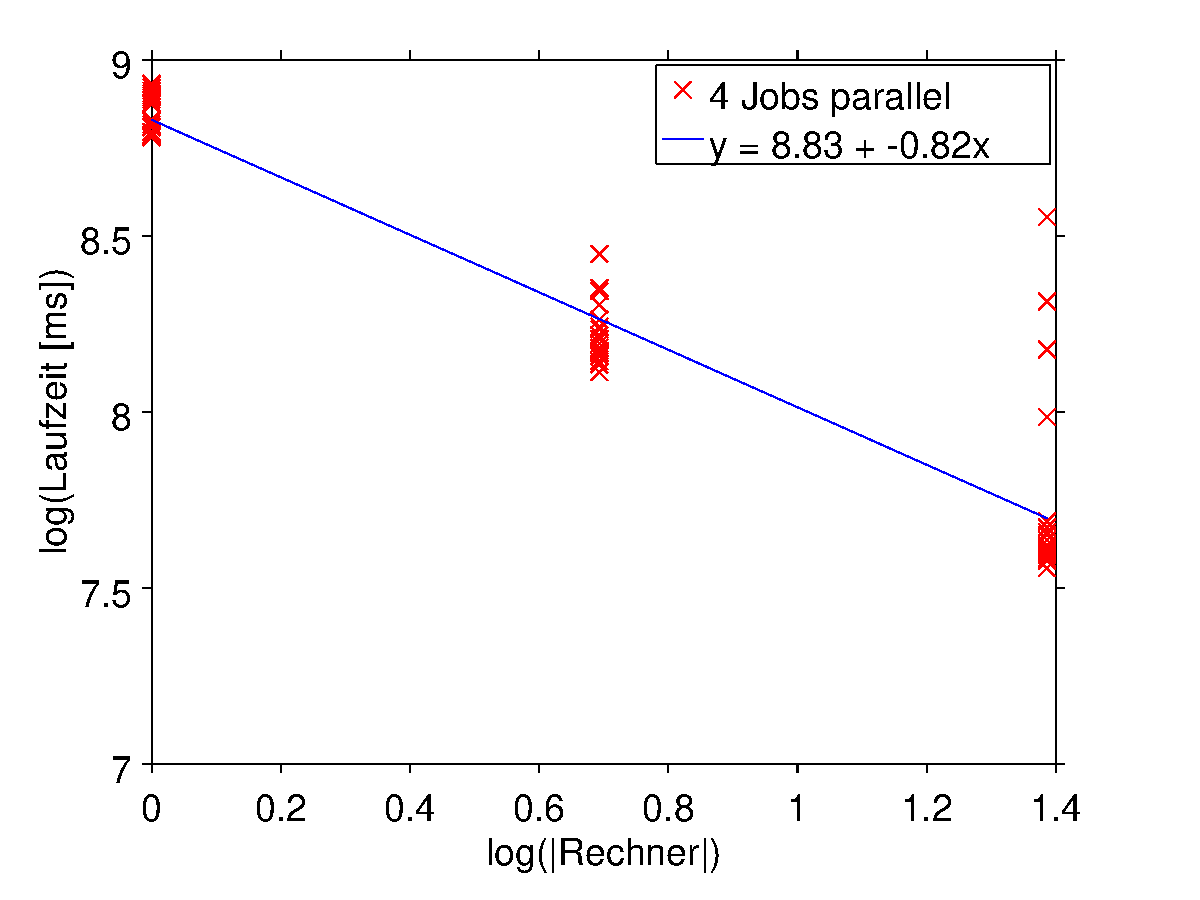
\includegraphics[width=\textwidth]{runtime-log-workerPrimeCpp}
    \caption{Experiment \ref{M1} Gesamtlaufzeiten mit 1, 2, und 4 Workern, und je 25 Iterationen. X und Y Achse logaritmiert.}
    \label{runtime-log-workerPrimeCpp}
  \end{minipage}
\end{figure}
























\clearpage
\subsection{\rgAlgorithmus{} - Pool Workflow}
\label{M2}

\begin{wrapfigure}{r}{0.45\textwidth}
  \vspace{-30pt}
  \begin{center}
    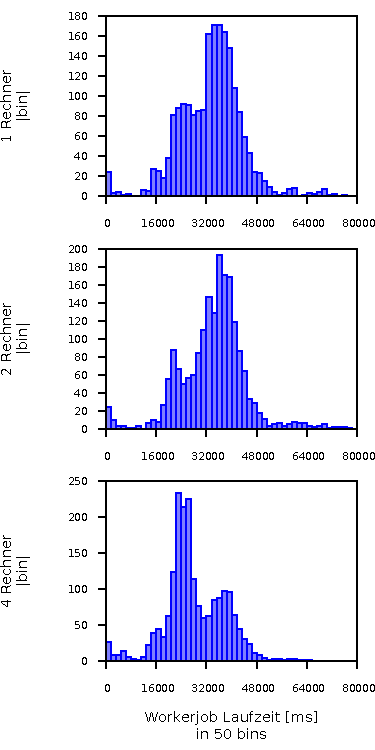
\includegraphics{hist-workerBacc0}
    \caption{Experiment \ref{M2} WorkerJob Laufzeiten aller 25 Iterationen in 50bins. Bei Pool Workflow sollte sich das Histogram nicht ändern.}
    \label{hist-workerBacc0}
  \end{center}
\end{wrapfigure}

Experiment 7.2 zeigt die verteilte Anwendung eines \rgAlgorithmus{}.
Jeder WorkerJob verarbeitet eine von 65 Input-Dateien mit Hilfe eines C++ Programms.
Input- und Output-Dateien werden auf ein AFS Dateisystem geschrieben.
Der Progress wird nur erhöht wenn die Verarbeitung einer Datei abgeschlossen wurde.
Dieses Experiment unterscheidet sich von Experiment \ref{M1} vor allem dadurch, dass deutlich mehr WorkerJobs erzeugt werden als Worker zur Verfügung stehen.
Für Laufzeiten siehe Tabelle \ref{testtable}.

Würde man die Anzahl der parallel laufenden WorkerJobs nicht  nach oben begrenzen, würde es zu Swapping kommen und die Gesamtlaufzeit verschlechtert sich.
Die Begrenzung der Anzahl an parallel laufenden WorkerJobs verhält sich wie Thread Pooling.
Theoretisch sollte dieses Script schlechter skalieren als \ref{M1}, da nach Terminierung eines WorkerJobs ein Roundtrip notwendig ist um den nächsten WorkerJob zu starten.
Insgesamt sind im Vergleich zu Experiment \ref{M1} $n - w$ zusätzliche Roundtrips notwendig, wobei $n$ die Anzahl der WorkerJobs, und $w$ die Anzahl der Worker ist.
Dieser Nachteil macht sich in der Gesamtlaufzeit allerdings kaum bemerkbar, solange ein WorkerJob (wie in diesem Fall) viel länger dauert als ein Roundtrip.

Ein weiterer Grund, warum dieses Experiment schlechter skaliert als Experiment \ref{M1}, ist die ungleiche Verteilung der WorkerJob Laufzeiten.
Wird der WorkerJob mit der längsten Laufzeit als letzter gestartet, wird dieser noch laufen, wenn alle anderen bereits terminiert haben
- oder anders gesagt, es werden nicht alle Ressourcen über die gesamte Laufzeit des Algorithmus genutzt (siehe Abschnitt \ref{schedulerNeeded}).
Sind die Laufzeiten der WorkerJobs im Voraus bekannt, könnte dieses Problem minimiert werden.


\vspace*{\fill}

\begin{figure}[H]
  \centering
  \begin{minipage}[b]{0.45\textwidth}
    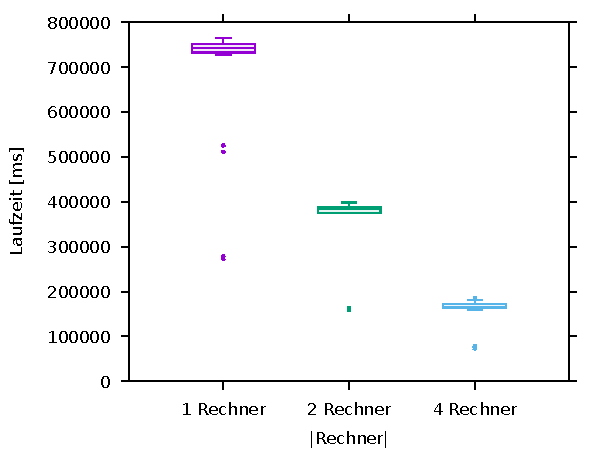
\includegraphics[width=\textwidth]{runtime-box-workerBacc0}
    \caption{Experiment \ref{M2}. Boxplots für Gesamtlaufzeit mit 1, 2, und 4 Worker, und je 25 Iterationen}
    \label{runtime-box-workerBacc0}
  \end{minipage}
  \hfill
  \begin{minipage}[b]{0.45\textwidth}
    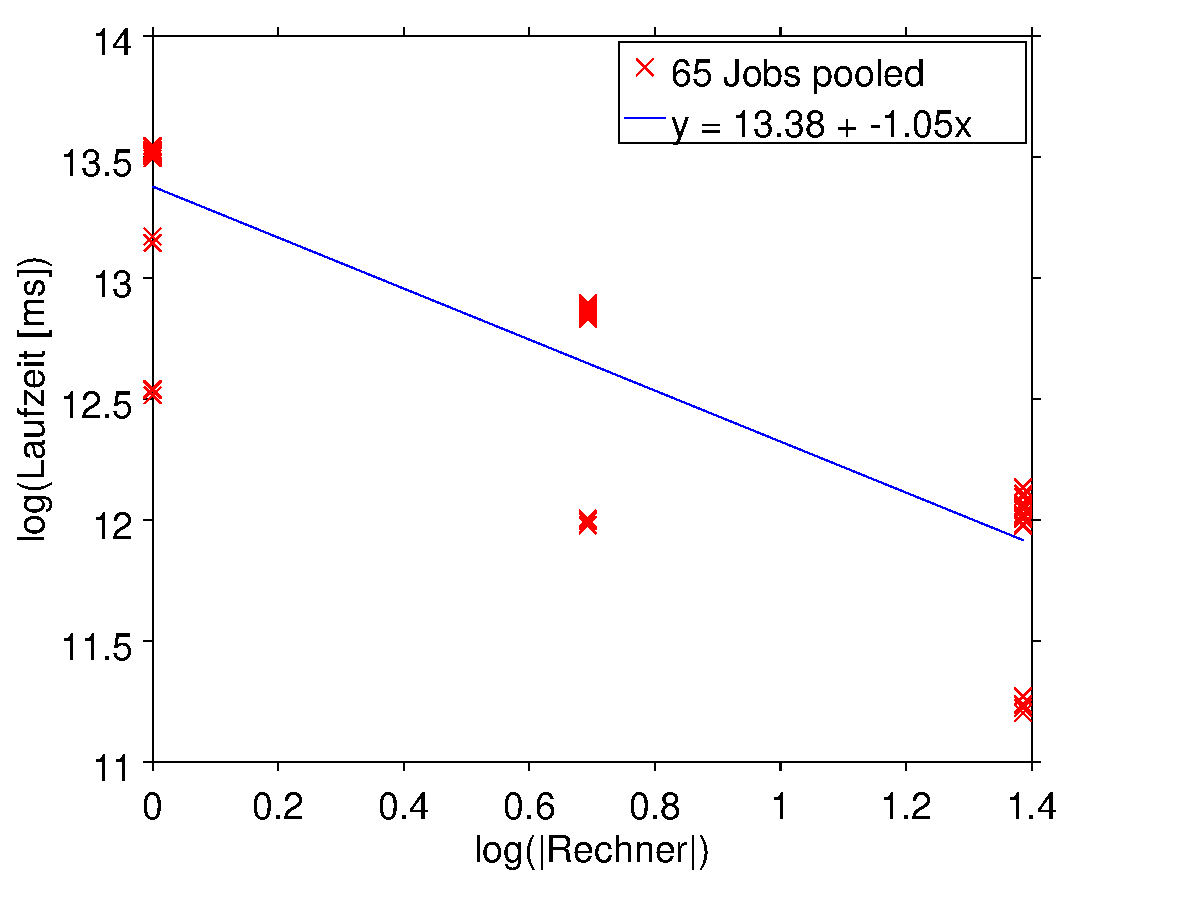
\includegraphics[width=\textwidth]{runtime-log-workerBacc0}
    \caption{Experiment \ref{M2} Gesamtlaufzeiten mit 1, 2, und 4 Workern, und je 25 Iterationen. X und Y Achse logaritmiert.}
    \label{runtime-log-workerBacc0}
  \end{minipage}
\end{figure}



















\clearpage
\subsection{Empty Jobs - Pool Workflow}
\label{M3}

\begin{wrapfigure}{r}{0.45\textwidth}
  \vspace{-30pt}
  \begin{center}
    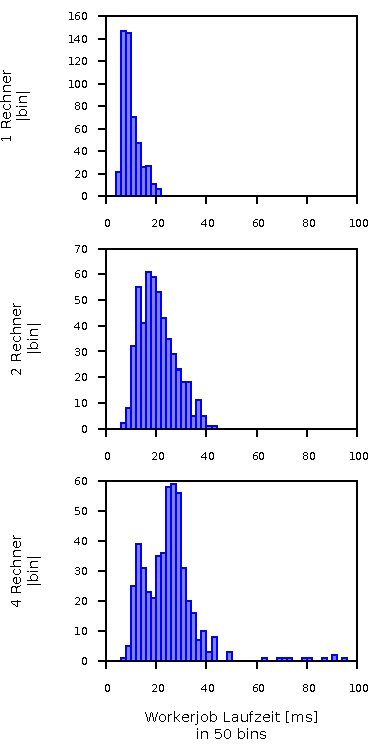
\includegraphics{hist-workerBacc1}
    \caption{Experiment \ref{M3} WorkerJob Laufzeiten aller 25 Iterationen in 50bins.  Bei Pool Workflow sollte sich das Histogram nicht ändern.}
    \label{hist-workerBacc1}
  \end{center}
\end{wrapfigure}

Dieses Experiment soll den durch die Middleware verursachten Overhead bei Verwendung eines Pool Workflows zeigen.
Die im Pool gestarteten WorkerJobs führen keinen Nutz-Algorithmus aus, sie terminieren unmittelbar nach dem Start.
Für Laufzeiten siehe Tabelle \ref{testtable}.
Wie alle anderen Experimente wird auch dieses mit einem, zwei und vier Rechnern mit je vier Workern ausgeführt.

Es zeigt sich, dass der Server bereits mit acht Workern, überlastet ist.
Zu erkennen ist dies am Histogramm in Abbildung \ref{hist-workerBacc1}.
Die Laufzeit von \remoteJob s wird am auftraggebenenden Gerät gemessen, inklusive Roundtrip, Serialisierung, und Workflow Logic.
Das Histogramm zeigt schon bei acht, und vor allem bei 16 Workern viel längere Laufzeiten.
Da die tatsächliche Laufzeit am Worker nahezu null ist und angenommen werden kann, dass die Roundtrip Zeit sich nicht wesentlich veränert hat, muss die zusätzliche Laufzeit dem Server zugeschrieben werden.

Die Message Sequenz ist die selbe wie bei \ref{M2}.
Gleicher Workflow bedeutet immer gleiche Message Sequenz mit Ausnahme der \UpdateMessage s, die hier vernachlässigt werden können.
Die Zeitabstände sind aber geringer, da die WorkerJobs sofort Terminieren.
Erhält der Server von zu vielen Workern Return Messages in kurzen Abständen, wächst die Queue am Server.
Die Auslastung des Servers ist von der Anzahl der Worker, die mit ihm verbunden sind, linear abhängig.
Ein \hcsno{} mit mehreren Worker Ebenen könnte dieses Problem beheben, da es die Serverauslastung logarithmisch von der Gesamtanzahl der Worker abhängig macht.
Ein solches System könnte in einer zukünftgien Arbeit untersucht werden.

\vspace*{\fill}

\begin{figure}[H]
  \centering
  \begin{minipage}[b]{0.45\textwidth}
    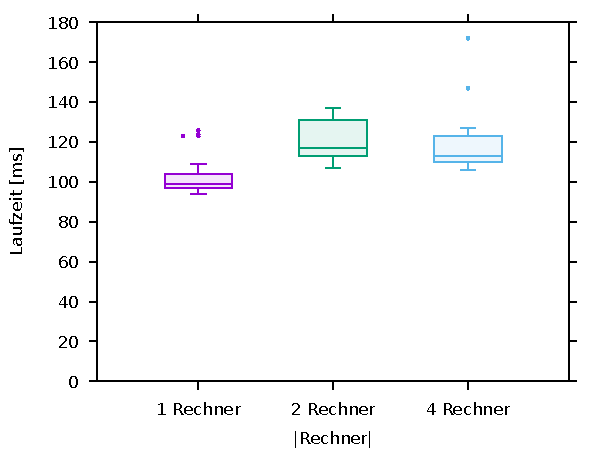
\includegraphics[width=\textwidth]{runtime-box-workerBacc1}
    \caption{Experiment \ref{M3}. Boxplots für Gesamtlaufzeit mit 1, 2, und 4 Worker, und je 25 Iterationen}
    \label{runtime-box-workerBacc1}
  \end{minipage}
  \hfill
  \begin{minipage}[b]{0.45\textwidth}
    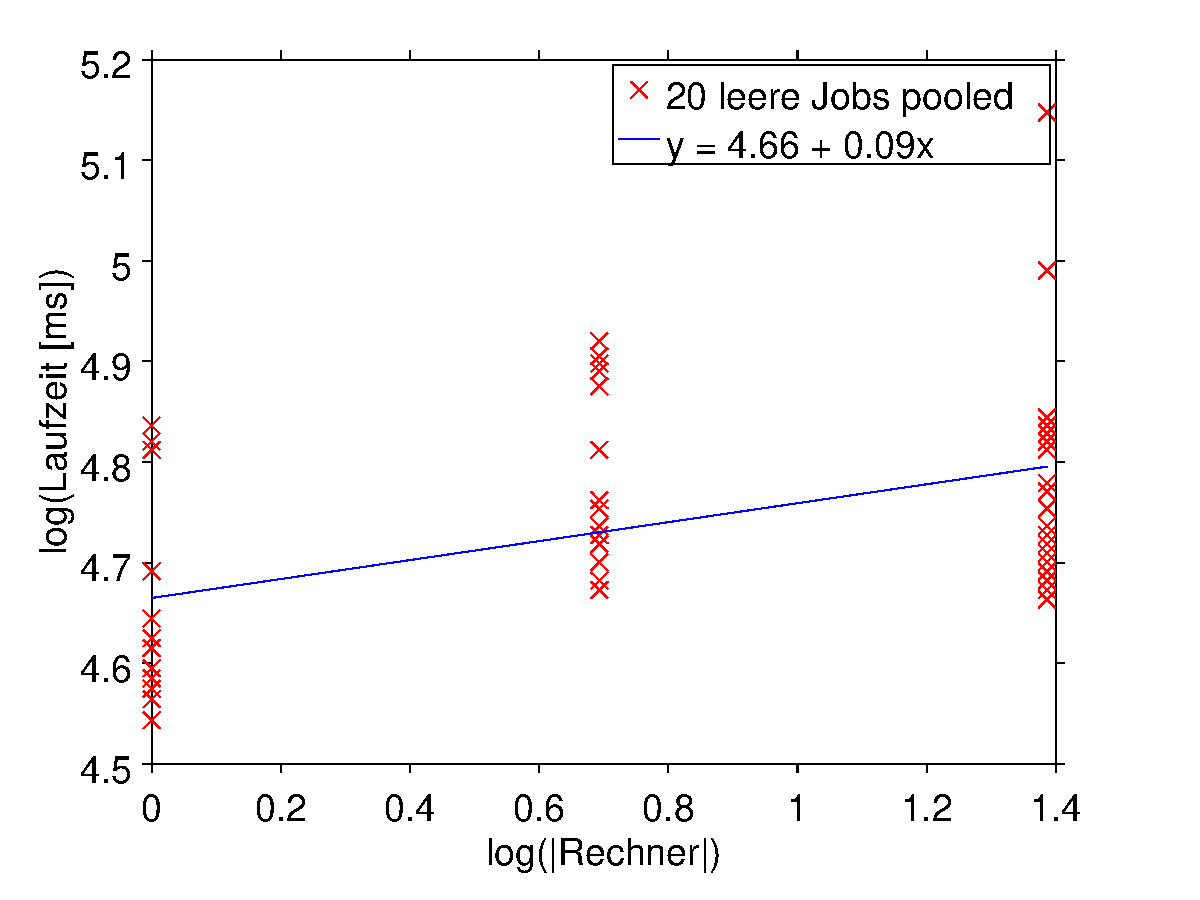
\includegraphics[width=\textwidth]{runtime-log-workerBacc1}
    \caption{Experiment \ref{M3} Gesamtlaufzeiten mit 1, 2, und 4 Workern, und je 25 Iterationen. X und Y Achse logaritmiert.}
    \label{runtime-log-workerBacc1}
  \end{minipage}
\end{figure}





















\clearpage
\section{Webclient Tests}
\subsection{\scheduler{} Fail}
\label{schedulerNeeded}
Folgendes Script führt 12 WorkerJobs mit zufälliger Laufzeit zwischen einer und 15 Sekunden in einem Pool von drei Workern aus.

Die Summe der Worker Laufzeiten beträgt 49s, durch die Anzahl der Worker geteilt sollte die Gesamtlaufzeit 17s nicht überschreiten.
Die Laufzeit beträgt aber 21s (siehe Tabelle \ref{testtable}), das System war also zu weniger als 84\% ausgelastet.
Abbildung \ref{fig:gant0} zeigt die nicht genutzten Worker Ressourcen im Gant Chart.
Ungünsige Konstellationen können eine noch weitaus schlechtere Auslastung zur Folge haben.
Bei unregelmäßigen WorkerJob Laufzeiten können andere \scheduler -Implementierungen für eine bessere Auslastung sorgen.
Das \scheduler{} Interface hat derzeit die Einschränkung, dass die Worker Nodes beim Start des Workflows bekannt sein müssen.

\begin{figure}[H]
  \begin{center}
    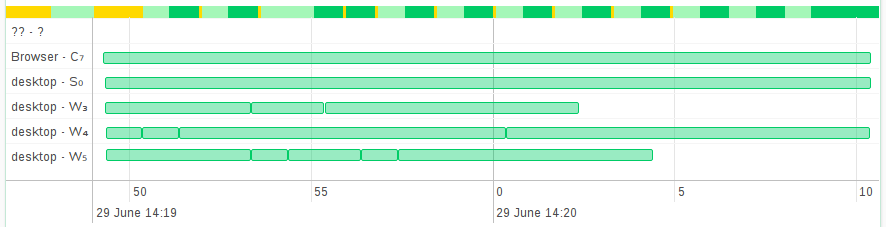
\includegraphics[width=1\textwidth]{gant}
    \caption{Gant Chart von 12 Workerjobs mit zufälliger Laufzeit.
    \label{fig:gant0}
    $W_4$ verzögert den Abschluss von $S_0$ und $C_7$ und verursacht dadurch eine und schlechte Systemauslastung. Diese Abbildung ist ein Screenshot des Webclients.}
  \end{center}
\end{figure}
\noindent



\subsection{Client Überlastung}
\label{overload}
Folgendes Script führt 20 ‘leere’ WorkerJobs in einem Pool von drei Workers aus.
Es ist das selbe Script das in Experiment \ref{M3} verwendet wurde.
Experiment \ref{M3} hat gezeigt, dass der CLI-Client leere Jobs mit bis zu 4 Worker Nodes verarbeiten kann.
Dieses Experiment wird mit 3 Worker Nodes ausgeführt, um eine Überlastung des Servers auszuschließen.

Am Webclient benötigt es 1064ms, der CLI-Client nur 103ms.
Der Webclient muss überlastet sein, da der Rest des Systems sich nicht geändert hat.
Auf den ersten Blick lässt Abbildung \ref{fig:gant2} vermuten, dass der Server überlastet ist.
Berücksichtigt man aber das $S_0$ am Client erstellt wurde, und Laufzeiten immer auf dem erstellenden Device gemessen werden, kann diese Fehlinterpretation erklärt werden.
Der Webclient ist, auch wenn die Anzahl der Worker korrekt dimensioniert wurde, anfällig für Überlastungen da \GUI{} Aktualisierungen rechenintensiv sind.


%Kurz nachdem der letzte WorkerJob auf $W_4$ terminiert, terminiert der ServerJob $S_0$ und danach der \RootJob{} am $C_7$.
%Die Verzögerung, bestehend aus Netzwerklatenz und Verarbeitungszeit der return Transition, ist minimal - in dieser Darstellung kaum sichtbar im Vergleich zu \ref{overload}.
%'Leer' bedeutet sie terminieren direkt nach dem Start. TODO |msg|=const -> runtime gering -> overhead macht maximialen teil aus.
%Abbildung \ref{fig:gant2} zeigt eine Überlastung des Clients oder Servers, erkennbar an der großen Zeitspanne zwischen dem Ende des letzten WorkerJobs und dem Ende des ServerJobs.
%Diese Verzögerung setzt sich zusammen aus Netzwerklatenz und onReturn Transition Verarbeitung, jeweils für den Server und Client - auf Server und Client, weil der auf $S_0$ ausgeführte Job auf $C_7$ erstellt wurde und die Joblaufzeit am auftraggebenden Gerät gemessen wird.
%Ob die Verzögerung auf dem Server oder Client entstanden ist, kann anhand dieses Diagramms nicht bestimmt werden.
%Eine Erweiterung der Visualisierung, die die Queueläge zeigt, würde die Identifizierung des überlasteten Geräts ermöglichen.
\begin{figure}[H]
  \begin{center}
    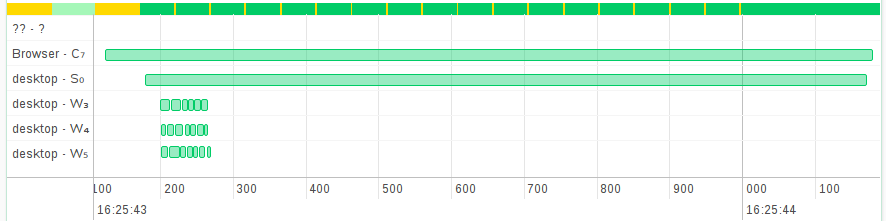
\includegraphics[width=1\textwidth]{gant2}
    \caption{Gant Chart von 20 Workerjobs mit minimaler Laufzeit.
    \label{fig:gant2}
    Das Scheduling der WorkerJobs ist akzeptabel. $C_7$ terminiert spät aufgrund einer Überlastung des Webclients. Diese Abbildung ist ein Screenshot des Webclients.}
  \end{center}
\end{figure}
\noindent

% =========================================================================
% CHAPTER 6
% =========================================================================

\chapter{Diskussion}
\label{K6}

\section{Fazit}
Der folgende Abschnitt diskutiert die Vor- und Nachteile von
on demand verteilten JobScripts,
der tiefen Position der Middleware im Schichtenmodel,
dem asyncronen Job API,
dem \JobTree{} Konzept
und der \UI{} Anbindung.


\begin{multicols}{2}
\subsection{Code on demand}
Die Implementierung hat gezeigt, dass die gewählten Technologien gut geeignet sind, um on demand verteilte Scripts von der Middleware ausführen zu lassen.
Der on demand verteilte Code eröffnet jedoch Angriffsmöglichkeiten.
Ein möglicher Lösungsansatz wären abgesicherte Sandboxes am Server und den Workern, wobei bedacht werden muss, dass das Starten von Prozessen ein gewünschtes Feature ist.
Die Verwendung von Secure Websockets, einer Benutzeranmeldung am Client und eine Assoziation der Websocket Verbindung mit einem Benutzer am Server wäre ebenso denkbar.
Dabei ist jedoch zu beachten, dass für jeden Benutzer des Webservers auch ein Benutzer im Betriebssystem angelegt werden muss.


\subsection{Jobs und Promises}
Das asynchrone API ist geeignet um Roundtrip arme \jobScript s zu schreiben, allerdings auch komplizierter als ein synchrones.
Die Ahnlichkeit zu \JavaScript{} Promises könnte zu einer Kompartiblität ausgebaut werden.
Jeder Job kann mit einem Timeout versehen werden.
Netzwerkprogrammierung erfordert häufig die Berücksichtigung von Timeouts, meist im Zusammenhang mit asynchronen Vorgängen.
Die Vereinigung dieser beiden Features in einer Klasse ermöglicht eine kompakte Implementierung der Requirments mit 1316 Zeilen JavaScript.
Timeouts finden auch bei lokalen asynchronen Operationen Anwendung.
Bei Promises kann man zwar Hardware Fehler vernachlässigen, aber Implementierungsfehler, wie zum Beispiel das fehlende Schließen einer Promise wird nicht erkannt.
Eine solche fehlerhafte Implementierung wird bei Jobs ein Timeout auslösen, was die Fehlersuche erleichtert.

\subsection{Low-level}
Das Middleware API ist auf einer tiefen Ebene im Schichtenmodell angesiedelt.
Daraus resultiert, dass Scheduler Algorithmen (\ref{schedulerNeeded}), Vermeidung von Überlastungen (\ref{overload}) und Workflow Logiken im \ApplicationLayer{} realisiert werden müssen.
Um diesen Umstand zu verbessern, könnten weitere Layer darüber geschaffen werden,
zum Beispiel nach dem Vorbild von \MapReduce{} oder \ApacheSpark{}.

\subsection{\JobTree s}
Mit der Hilfe der Job.delegate Funktion können Abhängigkeiten zwischen den Jobs deklariert werden.
Die Middleware kann so zur Laufzeit einen \JobTree{} aufbauen, der zu Debugging und Usability Zwecken verwendet werden kann.
Zum Beispiel ist im Fehlerfall daraus ersichtlich, auf welchem Gerät der Fehler stattgefunden hat.
Auch Ablaufvisualisierungen und Performance-Analysen sind damit möglich.

\subsection{\UI{} Anbindung}
Die onUpdate und onReturn Events der \RootJob s können für die Anbindung des \UI{} verwendet werden.
Die Anbindung ist sehr einfach, da die beiden Events alle durch das Netzwerk veruhrsachten \UI{} Updates abdecken (siehe Abbildung \ref{seq}).
Das gilt für das Anzeigen von Ergebnissen genauso wie für die Anzeige des Progress, Enablen/Disable Events und Fehlermeldungen - egal ob lokal oder remote.
Cancel Implementierungen sind vereinfacht auf das triviale Auslösen eines Abbruchs mit einem Funktionsaufruf.
Fehlermeldungen können ebenfalls im \UI{} dargestellt werden, indem im onReturn Event auf die Zustände der SubJobs geachtet wird.
\end{multicols}


%\item Der Anwender ist in der Lage, beliebige Verteilungsstrategien mit Hilfe von \jobScript s zu definieren, ohne einen Deployment Process auszuführen.
%Das Skript wird während der Ausführung an die entsprechenden Geräte verteilt - dies könnte auch als Deployment zur Runtime gesehen werden - jedenfalls geschieht es automatisch.
%\section{\RootJob{} Events und \UI{}}


\clearpage
%\section{Konklusion}
%\chapter{Fazit}
\section{Zukünftige Arbeiten}

Es wurden \jobScript s für zwei Network Overlays implementiert, Client Server und \hcsno{} mit einer Worker Ebene.
Für diese Overlays wurden jeweils mehrere Test Scripts mit geringem Zeitaufwand  implementiert.
Das Konzept könnte Anwendung bei der Implementierung von Prototypen finden.
Die Network Overlay Struktur ist vorerst aber noch statisch zur Runtime und eine Änderung würde die Anpassung von Kernkomponenten erfodern.
Eine Erweiterung um ein \ptp{} Network Overlay würde einen interessanten Raum für Experimente schaffen.


Kapitel \ref{K7} zeigt die Skalierbarkeit verschiedener Algorithmen verteilt auf ein \hcsno{} mit einer Worker Ebene.
Es ist ein grundlegendes Problem, dass ein Server nur eine begrenzte Anzahl von Workern bedienen kann.
Die \JavaScript{} Implementierung kann im worst Case Vier Worker pro Server bedienen (siehe \ref{M3}).
Eine sehr große Anzahl von Workern ist nur möglich, wenn nicht alle Worker mit demselben Server verbunden sind.
Ein hierarchisches Netzwerk mit mehreren Ebenen könnte für das Starten und Stoppen von Prozessen auf Worker eine Laufzeit  $T(n) = \mathcal{O}(log_{w}(n))$ erreichen, wobei $n$ die Gesamtanzahl der Worker und Server ist, und $w$ die Anzahl der Worker pro Server.
Auch die \ProgressAnzeige{} konnte dabei erhalten bleiben.


Derzeit enthält der Webclient mehrere Visualisierungen:
den Workflow Graph zu jedem Run eines Scripts, einen Gant Chart, der die Laufzeiten aller Jobs zeigt, sowie eine vereinfachte Darstellung des Netzwerks.
Sie alle visualisieren dasselbe Model, den \JobTree{}.
Für dieses Model könnten weitere Visualisierungen geschaffen werden, die bei Analysen helfen würden.
Der \JobTree{} könnte auch verwendet werden um mit Hilfe von Klassifikationsverfahren Fehler und Abweichungen zu erkennen.
Abbildung \ref{hist-workerBacc0} zeigt, dass einige WorkerJobs praktisch sofort termininierten, was auf ein Fehlverhalten hinweist.


Das Job API kann noch weiter vereinfacht werden.
Eine Kompatibilität zu JavaScript Promises würde bedeuten, dass Anwender die mit diesem schon vertraut sind, das Job API schnell erlernen würden.
Eine Trennung des Jobs in zwei Komponenten, Future und Promise nach \cite{baker1977incremental}, scheint aber auch sinnvoll.



%\item security
%\item onCall für ander programmirsprachen / onCall dependanxls

% ------------------------------------------------------------

\addcontentsline{toc}{chapter}{Bibliography}
\bibliographystyle{Scripts/eg-alpha}
\bibliography{Bibliography}
\addcontentsline{toc}{chapter}{List of Tables}
\listoftables
\addcontentsline{toc}{chapter}{List of Figures}
\listoffigures
\addcontentsline{toc}{chapter}{Index}
\twocolumn
\printindex

\end{document}
